\PassOptionsToPackage{enable-debug,check-declarations}{expl3}
\RequirePackage{pdfmanagement-testphase}
\DeclareDocumentMetadata {  }
\ExplSyntaxOn
\pdfmanagement_add:nnn{Catalog}{Lang}{(enUS)}
\ExplSyntaxOff

% xmp metadata for pdf
% Originally used \usepackage[a-2a]{pdfx}
% \usepackage{hyperxmp} replaced it
% \RequirePackage{pdfmanagement-testphase} replaced it

\documentclass[11pt,
  english,
  a4paper,
]{article}
\usepackage{sa4ss}
\usepackage{amsmath,amssymb,array}
\usepackage{booktabs}

% From tagged-template.latex
\usepackage{lmodern}
\usepackage{ifxetex,ifluatex}
\ifnum 0\ifxetex 1\fi\ifluatex 1\fi=0 % if pdftex
  \usepackage[T1]{fontenc}
  \usepackage[utf8]{inputenc}
  \usepackage{textcomp} % provide euro and other symbols
\else % if luatex or xetex
  \usepackage{unicode-math}
  \defaultfontfeatures{Scale=MatchLowercase}
  \defaultfontfeatures[\rmfamily]{Ligatures=TeX,Scale=1}
\fi

% Use upquote if available, for straight quotes in verbatim environments
\IfFileExists{upquote.sty}{\usepackage{upquote}}{}
\IfFileExists{microtype.sty}{% use microtype if available
  \usepackage[]{microtype}
  \UseMicrotypeSet[protrusion]{basicmath} % disable protrusion for tt fonts
}{}
\makeatletter
\@ifundefined{KOMAClassName}{% if non-KOMA class
  \IfFileExists{parskip.sty}{%
    \usepackage{parskip}
  }{% else
    \setlength{\parindent}{0pt}
    \setlength{\parskip}{6pt plus 2pt minus 1pt}}
}{% if KOMA class
  \KOMAoptions{parskip=half}}
\makeatother
\usepackage{xcolor}
\IfFileExists{xurl.sty}{\usepackage{xurl}}{} % add URL line breaks if available
\hypersetup{
  pdftitle={The status of Vermilion Rockfish (Sebastes miniatus) and Sunset Rockfish (Sebastes crocotulus) in U.S. waters off the coast of California north of Pt. Conception in 2021},
  pdflang={en},
  hidelinks,
  pdfcreator={LaTeX via pandoc}}
\urlstyle{same} % disable monospaced font for URLs
\usepackage{longtable}
% Correct order of tables after \paragraph or \subparagraph
\usepackage{etoolbox}
\makeatletter
\patchcmd\longtable{\par}{\if@noskipsec\mbox{}\fi\par}{}{}
\makeatother
% Allow footnotes in longtable head/foot
\IfFileExists{footnotehyper.sty}{\usepackage{footnotehyper}}{\usepackage{footnote}}
\makesavenoteenv{longtable}
\usepackage{graphicx}
\makeatletter
\def\maxwidth{\ifdim\Gin@nat@width>\linewidth\linewidth\else\Gin@nat@width\fi}
\def\maxheight{\ifdim\Gin@nat@height>\textheight\textheight\else\Gin@nat@height\fi}
\makeatother
% Scale images if necessary, so that they will not overflow the page
% margins by default, and it is still possible to overwrite the defaults
% using explicit options in \includegraphics[width, height, ...]{}
\setkeys{Gin}{width=\maxwidth,height=\maxheight,keepaspectratio}
% Set default figure placement to htbp
\makeatletter
\def\fps@figure{htbp}
\makeatother
\setlength{\emergencystretch}{3em} % prevent overfull lines
\providecommand{\tightlist}{%
  \setlength{\itemsep}{0pt}\setlength{\parskip}{0pt}}
\setcounter{secnumdepth}{5}
\usepackage{booktabs}
\usepackage{longtable}
\usepackage{array}
\usepackage{multirow}
\usepackage{wrapfig}
\usepackage{float}
\usepackage{colortbl}
\usepackage{pdflscape}
\usepackage{tabu}
\usepackage{threeparttable}
\usepackage[normalem]{ulem}
\usepackage{makecell}
\usepackage{xcolor}
\usepackage{placeins}
\ifxetex
  % Load polyglossia as late as possible: uses bidi with RTL langages (e.g. Hebrew, Arabic)
  \usepackage{polyglossia}
  \setmainlanguage[]{english}
\else
  \usepackage[shorthands=off,main=english]{babel}
\fi

%Define cslreferences environment, required by pandoc 2.8
%https://github.com/rstudio/rmarkdown/issues/1649
\newlength{\csllabelwidth}
\setlength{\csllabelwidth}{3em}
\newlength{\cslhangindent}
\setlength{\cslhangindent}{1.5em}
% for Pandoc 2.8 to 2.10.1
\newenvironment{cslreferences}%
  {}%
  {\par}
% For Pandoc 2.11+
\newenvironment{CSLReferences}[2] % #1 hanging-ident, #2 entry spacing
 {% don't indent paragraphs
  \setlength{\parindent}{0pt}
  % turn on hanging indent if param 1 is 1
  \ifodd #1 \everypar{\setlength{\hangindent}{\cslhangindent}}\ignorespaces\fi
  % set entry spacing
  \ifnum #2 > 0
  \setlength{\parskip}{#2\baselineskip}
  \fi
 }%
 {}
\usepackage{calc}  % for \widthof, \maxof in minipage
\newcommand{\CSLBlock}[1]{#1\hfill\break}
\newcommand{\CSLLeftMargin}[1]{\parbox[t]{\csllabelwidth}{#1}}
\newcommand{\CSLRightInline}[1]{\parbox[t]{\linewidth - \csllabelwidth}{#1}\break}
\newcommand{\CSLIndent}[1]{\hspace{\cslhangindent}#1}


\providecommand{\tightlist}{%
  \setlength{\itemsep}{0pt}\setlength{\parskip}{0pt}}

\usepackage{booktabs}
\usepackage{longtable}
\usepackage{array}
\usepackage{multirow}
\usepackage{wrapfig}
\usepackage{float}
\usepackage{colortbl}
\usepackage{pdflscape}
\usepackage{tabu}
\usepackage{threeparttable}
\usepackage[normalem]{ulem}
\usepackage{makecell}
\usepackage{xcolor}
\usepackage{placeins}
\date{}
\newcommand{\trTitle}{The status of Vermilion Rockfish (\emph{Sebastes miniatus}) and Sunset Rockfish (\emph{Sebastes crocotulus}) in U.S. waters off the coast of California north of Pt. Conception in 2021}
\newcommand{\trYear}{2021}
\newcommand{\trMonth}{June}
\newcommand{\trAuthsLong}{truetruetruetrue}
\newcommand{\trAuthsBack}{Monk, M.H., E.J. Dick, J.C. Field, E.M. Saas}
\newcommand{\trCitation}{
\begin{hangparas}{1em}{1}
\trAuthsBack{}. \trYear{}. \trTitle{}. Pacific Fisheries Management Council, Portland, Oregon. \pageref{LastPage}{}\,p.
\end{hangparas}}

\AtBeginDocument{\tagstructbegin{tag=Document}}
\AtEndDocument{\tagstructend}
\pretocmd{\maketitle}{\tagstructbegin{tag=H1}\tagmcbegin{tag=H1}}{}{}
\apptocmd{\maketitle}{\tagmcend\tagstructend}{}{}

\begin{document}

%%%%% Frontmatter %%%%%

% Footnote symbols in front matter
\renewcommand*{\thefootnote}{\fnsymbol{footnote}}

\small
\thispagestyle{empty}
\pagenumbering{roman}
\noindent
\begin{center}
\title{The status of Vermilion Rockfish (\emph{Sebastes miniatus}) and Sunset Rockfish (\emph{Sebastes crocotulus}) in U.S. waters off the coast of California north of Pt. Conception in 2021}
% \textnormal{\MakeTextUppercase{\trTitle{}}}
\vspace{1.5cm}
{\Large\textbf\newline{The status of Vermilion Rockfish (\emph{Sebastes miniatus}) and Sunset Rockfish (\emph{Sebastes crocotulus}) in U.S. waters off the coast of California north of Pt. Conception in 2021}}
\vfill
by\\
Melissa H. Monk\textsuperscript{1}\\
E. J. Dick\textsuperscript{1}\\
John C. Field\textsuperscript{1}\\
Emma M. Saas\textsuperscript{1}\vfill
\textsuperscript{1}Southwest Fisheries Science Center, U.S. Department of Commerce, National Oceanic and Atmospheric Administration, National Marine Fisheries Service, 110 McAllister Way, Santa Cruz, California 95060\vfill
\trMonth{} \trYear{}
\end{center}
\clearpage

% Fourth page: Colophon
\thispagestyle{empty}
\vspace*{\fill}
\begin{center}
\copyright{} Pacific Fisheries Management Council, \trYear{}\\
\end{center}
\par
\bigskip
\noindent
Correct citation for this publication:
\bigskip
\par
\trCitation{}
\clearpage

% Add TOC to pdf bookmarks (clickable pdf)
\pdfbookmark[1]{\contentsname}{toc}

% Table of contents page, lists of figures and tables
\tableofcontents\clearpage
\label{TRlastRoman}
\clearpage

% Table of contents
\newpage
\thispagestyle{empty} % to remove page number

% Settings for the main document
\pagenumbering{arabic}  % Regular page numbers
\pagestyle{plain}  % No page number on first page of main document, use 'empty'
\renewcommand*{\thefootnote}{\arabic{footnote}}  % Back to numeric footnotes
\setcounter{footnote}{0}  % And start at 1
\renewcommand{\headrulewidth}{0.5pt}
\renewcommand{\footrulewidth}{0.5pt}
%\pagestyle{fancy}\fancyhead[c]{Draft: Do not cite or circulate}

\newcommand{\lt}{\ensuremath <}
\newcommand{\gt}{\ensuremath >}

\pagebreak
\pagenumbering{roman}
\setcounter{page}{1}

\renewcommand{\thetable}{\roman{table}}
\renewcommand{\thefigure}{\roman{figure}}

\setlength\parskip{0.5em plus 0.1em minus 0.2em}

\tagstructbegin{tag=H1}\tagmcbegin{tag=H1}

\hypertarget{executive-summary}{%
\section*{Executive Summary}\label{executive-summary}}
\addcontentsline{toc}{section}{Executive Summary}

\leavevmode\tagmcend\tagstructend

To be completed after the STAR panel.

\tagstructbegin{tag=H2}\tagmcbegin{tag=H2}

\hypertarget{stock}{%
\subsection*{Stock}\label{stock}}
\addcontentsline{toc}{subsection}{Stock}

\leavevmode\tagmcend\tagstructend

This assessment reports the status of the vermlion rockfish (\emph{Sebastes miniatus}) and sunset rockfish (\emph{Sebastes crocotulus}) complex (referred to as vermilion throughout), resource in U.S. waters off the coast of California north of Point Conception ({\tagstructbegin{tag=Formula}\tagmcbegin{tag=Formula}\(34^\circ 27^\prime\)\leavevmode\tagmcend\tagstructend} N. latitude) using data through 2020.

\tagstructbegin{tag=H2}\tagmcbegin{tag=H2}

\hypertarget{landings}{%
\subsection*{Landings}\label{landings}}
\addcontentsline{toc}{subsection}{Landings}

\leavevmode\tagmcend\tagstructend

Replace text.

\tagstructbegin{tag=H2}\tagmcbegin{tag=H2}

\hypertarget{data-and-assessment}{%
\subsection*{Data and Assessment}\label{data-and-assessment}}
\addcontentsline{toc}{subsection}{Data and Assessment}

\leavevmode\tagmcend\tagstructend

Replace text.

\tagstructbegin{tag=H2}\tagmcbegin{tag=H2}

\hypertarget{stock-biomass}{%
\subsection*{Stock Biomass}\label{stock-biomass}}
\addcontentsline{toc}{subsection}{Stock Biomass}

\leavevmode\tagmcend\tagstructend

Replace text.

\tagstructbegin{tag=H2}\tagmcbegin{tag=H2}

\hypertarget{recruitment}{%
\subsection*{Recruitment}\label{recruitment}}
\addcontentsline{toc}{subsection}{Recruitment}

\leavevmode\tagmcend\tagstructend

Replace text.

\tagstructbegin{tag=H2}\tagmcbegin{tag=H2}

\hypertarget{exploitation-status}{%
\subsection*{Exploitation Status}\label{exploitation-status}}
\addcontentsline{toc}{subsection}{Exploitation Status}

\leavevmode\tagmcend\tagstructend

Replace text.

\tagstructbegin{tag=H2}\tagmcbegin{tag=H2}

\hypertarget{reference-points}{%
\subsection*{Reference Points}\label{reference-points}}
\addcontentsline{toc}{subsection}{Reference Points}

\leavevmode\tagmcend\tagstructend

Replace text.

\tagstructbegin{tag=H2}\tagmcbegin{tag=H2}

\hypertarget{management-performance}{%
\subsection*{Management Performance}\label{management-performance}}
\addcontentsline{toc}{subsection}{Management Performance}

\leavevmode\tagmcend\tagstructend

Replace text.

\tagstructbegin{tag=H2}\tagmcbegin{tag=H2}

\hypertarget{unresolved-problems-and-major-uncertainties}{%
\subsection*{Unresolved Problems and Major Uncertainties}\label{unresolved-problems-and-major-uncertainties}}
\addcontentsline{toc}{subsection}{Unresolved Problems and Major Uncertainties}

\leavevmode\tagmcend\tagstructend

Replace text.

\tagstructbegin{tag=H2}\tagmcbegin{tag=H2}

\hypertarget{decision-table}{%
\subsection*{Decision Table}\label{decision-table}}
\addcontentsline{toc}{subsection}{Decision Table}

\leavevmode\tagmcend\tagstructend

Replace text.

\tagstructbegin{tag=H2}\tagmcbegin{tag=H2}

\hypertarget{research-and-data-needs}{%
\subsection*{Research and Data Needs}\label{research-and-data-needs}}
\addcontentsline{toc}{subsection}{Research and Data Needs}

\leavevmode\tagmcend\tagstructend

Replace text.

\pagebreak
\setlength{\parskip}{5mm plus1mm minus1mm}
\pagenumbering{arabic}
\setcounter{page}{1}
\renewcommand{\thefigure}{\arabic{figure}}
\renewcommand{\thetable}{\arabic{table}}
\setcounter{table}{0}
\setcounter{figure}{0}

\tagstructbegin{tag=H1}\tagmcbegin{tag=H1}

\hypertarget{introduction}{%
\section{Introduction}\label{introduction}}

\leavevmode\tagmcend\tagstructend

\tagstructbegin{tag=H2}\tagmcbegin{tag=H2}

\hypertarget{basic-information}{%
\subsection{Basic Information}\label{basic-information}}

\leavevmode\tagmcend\tagstructend

This assessment reports the status of the Vermilion Rockfish (\emph{Sebastes miniatus}) and Sunset Rockfish (\emph{Sebastes crocotulus}) in U.S. waters off the coast of California south of Pt. Conception through 2020.

\#\#Basic Information and Life History

\emph{Population Structure and Complex Assessment Considerations}

Provided by John Harms (NWFSC)

A group of researchers from the NWFSC and SWFSC is collaborating on a project to genotype tissue specimens collected from the vermilion and sunset rockfish cryptic pair captured during the West Coast Groundfish Bottom Trawl Survey and the Southern CA Shelf Rockfish Hook and Line Survey for the years 2004 - 2019. Funding for this project was obtained through the Saltonstall-Kennedy program for FY 2020 through a proposal led by representatives from Pacific States Marine Fisheries Commission and the commercial passenger fishing vessel industry in southern California.

After combining with specimens obtained through other collection efforts along the West Coast, approximately 25,000 tissue specimens will be analyzed. Some earlier efforts to separate this cryptic pair to species used mitochondrial DNA (mtDNA) markers. However, due to a one-way mitochondrial introgression from the vermilion genome into the sunset genome, a portion of the sunset rockfish population contains mitochondrial DNA sequences consistent with vermilion rockfish resulting in incorrect species assignments for these introgressed individuals during the prior research project. The current research has identified a robust suite of genetic markers within the nuclear genomes of the two species that definitively separates vermilion and sunset rockfish (including introgressed sunset rockfish), canary rockfish, first generation vermilion-sunset hybrids, and identifies emerging patterns of intraspecific stock structure within the two sister species.

Once the collected specimens have been genotyped, any species-specific differences in spatial and depth distribution, size composition, weight-length relationships, and other biological characteristics will be identified. Using previously collected otoliths and ovaries, the demographics of the two species including age and growth and reproductive biology parameters such as length and age at 50\% maturity and the prevalence of skip spawning will be explored and compared. These new genotyping results will be combined with data from the prior mtDNA work to evaluate whether introgressed sunset rockfish represent a biologically intermediate subform of the species complex. The effort also proposes to develop and test the efficacy of models to predict the relative proportion of the two species based upon explanatory variables including latitude, depth, species of co-occurrence, oceanographic parameters, habitat descriptors and/or other information. The anticipated completion of the genotyping of all specimens is approximately December 2021 with provision of final results by the end of FY 2022.

This research is aimed at providing information to support the successful stock assessment of this commercially and recreationally valuable cryptic species pair and is responsive to any data gaps identified by the assessment community. If successful, this research, conducted in close communication with stock assessors, may also assist the PFMC in establishing best practices for the assessment and management of cryptic species complexes. Though this project will only focus on nominal vermilion rockfish specimens collected through the 2019 survey field season, it may be advisable that tissue specimens collected aboard fishery-independent surveys as well as through fishery-dependent programs continue to be genotyped on an ongoing basis to support continued and timely monitoring of this economically and ecologically important species complex.

\tagstructbegin{tag=H2}\tagmcbegin{tag=H2}

\hypertarget{early-life-history}{%
\subsection{Early Life History}\label{early-life-history}}

\leavevmode\tagmcend\tagstructend

\#\#Map

\#\#Ecosystem Considerations

\tagstructbegin{tag=H2}\tagmcbegin{tag=H2}

\hypertarget{historical-and-current-fishery-information}{%
\subsection{Historical and Current Fishery Information}\label{historical-and-current-fishery-information}}

\leavevmode\tagmcend\tagstructend

Replace text.

\tagstructbegin{tag=H2}\tagmcbegin{tag=H2}

\hypertarget{summary-of-management-history-and-performance}{%
\subsection{Summary of Management History and Performance}\label{summary-of-management-history-and-performance}}

\leavevmode\tagmcend\tagstructend

Replace text.

\#\#Management Performance

\tagstructbegin{tag=H2}\tagmcbegin{tag=H2}

\hypertarget{foreign-fisheries}{%
\subsection{Foreign Fisheries}\label{foreign-fisheries}}

\leavevmode\tagmcend\tagstructend

Replace text.

\tagstructbegin{tag=H1}\tagmcbegin{tag=H1}

\hypertarget{data}{%
\section{Data}\label{data}}

\leavevmode\tagmcend\tagstructend

A description of each data source is provided below (Figure).

\tagstructbegin{tag=H2}\tagmcbegin{tag=H2}

\hypertarget{biological-data}{%
\subsection{Biological Data}\label{biological-data}}

\leavevmode\tagmcend\tagstructend

\tagstructbegin{tag=H3}\tagmcbegin{tag=H3}

\hypertarget{length-and-age-compositions}{%
\subsubsection{Length and Age Compositions}\label{length-and-age-compositions}}

\leavevmode\tagmcend\tagstructend

Differences in length compositions and length-at-age were explored north and south of Pt. Conception prior to any modelling. There are currently no available data to separate sunset and vermilion rockfishes.

Length compositions were provided from the following sources:

\emph{North of Pt. Conception}

\tagstructbegin{tag=L}

\begin{itemize}
\item
  \tagstructbegin{tag=LI}\tagstructbegin{tag=LBody}\tagmcbegin{tag=P}

  Commercial sources

  \tagmcend\tagstructend\tagstructend

  \tagstructbegin{tag=L}

  \begin{itemize}
  \item
    \tagstructbegin{tag=LI}\tagstructbegin{tag=LBody}\tagmcbegin{tag=P}

    \tagstructbegin{tag=LI}\tagstructbegin{tag=LBody}\tagmcbegin{tag=P}

    CALCOM (1978-2020)

    \tagmcend\tagstructend\tagstructend

    \tagmcend\tagstructend\tagstructend
  \end{itemize}

  \tagstructend
\item
  \tagstructbegin{tag=LI}\tagstructbegin{tag=LBody}\tagmcbegin{tag=P}

  Recreational sources

  \tagmcend\tagstructend\tagstructend

  \tagstructbegin{tag=L}

  \begin{itemize}
  \item
    \tagstructbegin{tag=LI}\tagstructbegin{tag=LBody}\tagmcbegin{tag=P}

    \tagstructbegin{tag=LI}\tagstructbegin{tag=LBody}\tagmcbegin{tag=P}

    Miller and Gotshall dockside survey (1959-1960)

    \tagmcend\tagstructend\tagstructend

    \tagmcend\tagstructend\tagstructend
  \item
    \tagstructbegin{tag=LI}\tagstructbegin{tag=LBody}\tagmcbegin{tag=P}

    \tagstructbegin{tag=LI}\tagstructbegin{tag=LBody}\tagmcbegin{tag=P}

    CPFV samples from Commercial port samplers (1978-1979)

    \tagmcend\tagstructend\tagstructend

    \tagmcend\tagstructend\tagstructend
  \item
    \tagstructbegin{tag=LI}\tagstructbegin{tag=LBody}\tagmcbegin{tag=P}

    \tagstructbegin{tag=LI}\tagstructbegin{tag=LBody}\tagmcbegin{tag=P}

    Deb Wilson-Vandenberg's onboard observer survey (1988-1998)

    \tagmcend\tagstructend\tagstructend

    \tagmcend\tagstructend\tagstructend
  \item
    \tagstructbegin{tag=LI}\tagstructbegin{tag=LBody}\tagmcbegin{tag=P}

    \tagstructbegin{tag=LI}\tagstructbegin{tag=LBody}\tagmcbegin{tag=P}

    MRFSS dockside survey (1980-2003)

    \tagmcend\tagstructend\tagstructend

    \tagmcend\tagstructend\tagstructend
  \item
    \tagstructbegin{tag=LI}\tagstructbegin{tag=LBody}\tagmcbegin{tag=P}

    \tagstructbegin{tag=LI}\tagstructbegin{tag=LBody}\tagmcbegin{tag=P}

    CRFS onboard and dockside survey (2004-2019)

    \tagmcend\tagstructend\tagstructend

    \tagmcend\tagstructend\tagstructend
  \end{itemize}

  \tagstructend
\item
  \tagstructbegin{tag=LI}\tagstructbegin{tag=LBody}\tagmcbegin{tag=P}

  Fishery-independent surveys

  \tagmcend\tagstructend\tagstructend

  \tagstructbegin{tag=L}

  \begin{itemize}
  \item
    \tagstructbegin{tag=LI}\tagstructbegin{tag=LBody}\tagmcbegin{tag=P}

    \tagstructbegin{tag=LI}\tagstructbegin{tag=LBody}\tagmcbegin{tag=P}

    CCFRP hook-and-line survey (2007-2018)

    \tagmcend\tagstructend\tagstructend

    \tagmcend\tagstructend\tagstructend
  \item
    \tagstructbegin{tag=LI}\tagstructbegin{tag=LBody}\tagmcbegin{tag=P}

    \tagstructbegin{tag=LI}\tagstructbegin{tag=LBody}\tagmcbegin{tag=P}

    West Coast Groundfish Bottown Trawl Survey (2003-2019)

    \tagmcend\tagstructend\tagstructend

    \tagmcend\tagstructend\tagstructend
  \end{itemize}

  \tagstructend
\end{itemize}

\tagstructend

\emph{South of Pt. Conception}

\tagstructbegin{tag=L}

\begin{itemize}
\item
  \tagstructbegin{tag=LI}\tagstructbegin{tag=LBody}\tagmcbegin{tag=P}

  Commercial sources

  \tagmcend\tagstructend\tagstructend

  \tagstructbegin{tag=L}

  \begin{itemize}
  \item
    \tagstructbegin{tag=LI}\tagstructbegin{tag=LBody}\tagmcbegin{tag=P}

    \tagstructbegin{tag=LI}\tagstructbegin{tag=LBody}\tagmcbegin{tag=P}

    CALCOM (1978-2020)

    \tagmcend\tagstructend\tagstructend

    \tagmcend\tagstructend\tagstructend
  \end{itemize}

  \tagstructend
\item
  \tagstructbegin{tag=LI}\tagstructbegin{tag=LBody}\tagmcbegin{tag=P}

  Recreational sources

  \tagmcend\tagstructend\tagstructend

  \tagstructbegin{tag=L}

  \begin{itemize}
  \item
    \tagstructbegin{tag=LI}\tagstructbegin{tag=LBody}\tagmcbegin{tag=P}

    \tagstructbegin{tag=LI}\tagstructbegin{tag=LBody}\tagmcbegin{tag=P}

    Ally et al.~onboard observer survey (1986-1989)

    \tagmcend\tagstructend\tagstructend

    \tagmcend\tagstructend\tagstructend
  \item
    \tagstructbegin{tag=LI}\tagstructbegin{tag=LBody}\tagmcbegin{tag=P}

    \tagstructbegin{tag=LI}\tagstructbegin{tag=LBody}\tagmcbegin{tag=P}

    Collins and Crooke onboard observer survey (1975-1978)

    \tagmcend\tagstructend\tagstructend

    \tagmcend\tagstructend\tagstructend
  \item
    \tagstructbegin{tag=LI}\tagstructbegin{tag=LBody}\tagmcbegin{tag=P}

    \tagstructbegin{tag=LI}\tagstructbegin{tag=LBody}\tagmcbegin{tag=P}

    MRFSS dockside survey (1980-2003)

    \tagmcend\tagstructend\tagstructend

    \tagmcend\tagstructend\tagstructend
  \item
    \tagstructbegin{tag=LI}\tagstructbegin{tag=LBody}\tagmcbegin{tag=P}

    \tagstructbegin{tag=LI}\tagstructbegin{tag=LBody}\tagmcbegin{tag=P}

    CRFS onboard and dockside survey (2004-2018)

    \tagmcend\tagstructend\tagstructend

    \tagmcend\tagstructend\tagstructend
  \end{itemize}

  \tagstructend
\item
  \tagstructbegin{tag=LI}\tagstructbegin{tag=LBody}\tagmcbegin{tag=P}

  Fishery-independent surveys

  \tagmcend\tagstructend\tagstructend

  \tagstructbegin{tag=L}

  \begin{itemize}
  \item
    \tagstructbegin{tag=LI}\tagstructbegin{tag=LBody}\tagmcbegin{tag=P}

    \tagstructbegin{tag=LI}\tagstructbegin{tag=LBody}\tagmcbegin{tag=P}

    NWFSC Hook-and-Line Survey (2004-2019)

    \tagmcend\tagstructend\tagstructend

    \tagmcend\tagstructend\tagstructend
  \item
    \tagstructbegin{tag=LI}\tagstructbegin{tag=LBody}\tagmcbegin{tag=P}

    \tagstructbegin{tag=LI}\tagstructbegin{tag=LBody}\tagmcbegin{tag=P}

    West Coast Groundfish Bottown Trawl Survey (2003-2019)

    \tagmcend\tagstructend\tagstructend

    \tagmcend\tagstructend\tagstructend
  \end{itemize}

  \tagstructend
\end{itemize}

\tagstructend

The length composition of all fisheries aggregated across time by fleet is in Figure \ref{fig:comp_lendat_aggregated_across_time} and Table xxx. Descriptions and details of the length composition data are in the above section for each fleet or survey.

\tagstructbegin{tag=H3}\tagmcbegin{tag=H3}

\hypertarget{age-structures}{%
\subsubsection{Age Structures}\label{age-structures}}

\leavevmode\tagmcend\tagstructend

\textbf{External Fits to Growth}

Fits to the von Bertalanffy growth curve, {\tagstructbegin{tag=Formula}\tagmcbegin{tag=Formula}\(L_i = L_{\infty}e^{(-k[t-t_0])}\)\leavevmode\tagmcend\tagstructend}, where {\tagstructbegin{tag=Formula}\tagmcbegin{tag=Formula}\(L_i\)\leavevmode\tagmcend\tagstructend} is the length (cm) at age {\tagstructbegin{tag=Formula}\tagmcbegin{tag=Formula}\(i\)\leavevmode\tagmcend\tagstructend}, {\tagstructbegin{tag=Formula}\tagmcbegin{tag=Formula}\(t\)\leavevmode\tagmcend\tagstructend} is age in years, {\tagstructbegin{tag=Formula}\tagmcbegin{tag=Formula}\(k\)\leavevmode\tagmcend\tagstructend} is rate of increase in growth, {\tagstructbegin{tag=Formula}\tagmcbegin{tag=Formula}\(t_0\)\leavevmode\tagmcend\tagstructend} is the intercept, and {\tagstructbegin{tag=Formula}\tagmcbegin{tag=Formula}\(L_{\infty}\)\leavevmode\tagmcend\tagstructend} is the asymptotic length, were explore by species and sex.

\tagstructbegin{tag=H3}\tagmcbegin{tag=H3}

\hypertarget{ageing-precision-and-bias}{%
\subsubsection{Ageing Precision and Bias}\label{ageing-precision-and-bias}}

\leavevmode\tagmcend\tagstructend

Uncertainty in ageing error was estimated using a collection of 357 vermilion rockfish otoliths with two age reads between the NWFSC (reader 1, B. Kamikawa) and the SWFSC (reader 2, D. Watters) (Figure \ref{fig:reader1reader2}). Age-composition data used in the model were from a number of sources described above. The same readers aged otoliths for both vermilion rockfish stock assessmetnt models. Age reader 1 read all of the otoliths for the southern model and both readers read otoliths for the northern California model. In addition to the otoliths from these two regions, the same two readers aged fish for a Committee of Age Reading Experts (CARE)exchange among four ageing labs, initiated by the SWFSC.

Ageing error was estimated using publicly available software {\tagstructbegin{tag=Reference}\tagmcbegin{tag=Reference}(Thorson, Stewart, and Punt 2012)\leavevmode\tagmcend\tagstructend}. The software setting for bias was set to unbiased for reader 1 who was more experienced. The {\tagstructbegin{tag=Formula}\tagmcbegin{tag=Formula}\(\Delta AIC\)\leavevmode\tagmcend\tagstructend} among the top three models was less than two. The best fitting model selected curvilinear bias for reader 1 and curvilinear standard deviation for both readers.\\
An analysis of ageing error removing one fish aged at 88 by reader 1 and 78 by reader 2 selected the the model with reader 2 as unbiased and curvilinear standard deviation (Figure \ref{fig:oldfish}). The reading of the oldest aged fish falls within the 95\% confidence internal using this model (Figure \ref{fig:truereads}).\\
The latter model was selected for use in the assessment.

The resulting estimate indicated a standard deviation in age readings increasing from 0.001 years at age 0 to a standard deviation of 2.37 years at age 70, the first year of the plus group in the assessment model.

\tagstructbegin{tag=H3}\tagmcbegin{tag=H3}

\hypertarget{maturation-and-fecundity}{%
\subsubsection{Maturation and Fecundity}\label{maturation-and-fecundity}}

\leavevmode\tagmcend\tagstructend

\tagstructbegin{tag=H3}\tagmcbegin{tag=H3}

\hypertarget{natural-mortality}{%
\subsubsection{Natural Mortality}\label{natural-mortality}}

\leavevmode\tagmcend\tagstructend

Natural mortality was not directly measured, so life-history based empirical relationships were used. The Natural Mortality Tool (NMT; {\tagstructbegin{tag=Link}\tagmcbegin{tag=Link}\url{https://github.com/shcaba/Natural-Mortality-Tool}\leavevmode\tagmcend\tagstructend}), a Shiny-based graphical user interface allowing for the application of a variety of natural mortality estimators based on measures such as longevity, size, age and growth, and maturity, was used to obtain estimates of natural mortality. The NMT currently provides 19 options, including the Hamel {\tagstructbegin{tag=Reference}\tagmcbegin{tag=Reference}(2015)\leavevmode\tagmcend\tagstructend} method, which is a corrected form of the Then et al. {\tagstructbegin{tag=Reference}\tagmcbegin{tag=Reference}(2018)\leavevmode\tagmcend\tagstructend} functional regression model and is a commomly applied method for west coast groundfish. The NMT also allows for the construction of a natural mortality prior weighted across methods by the user.

\tagstructbegin{tag=H3}\tagmcbegin{tag=H3}

\hypertarget{sex-ratio}{%
\subsubsection{Sex Ratio}\label{sex-ratio}}

\leavevmode\tagmcend\tagstructend

No information on the sex ratio at birth was available so it was assumed to be 50:50.

\tagstructbegin{tag=H3}\tagmcbegin{tag=H3}

\hypertarget{length-weight-relationship}{%
\subsubsection{Length-Weight Relationship}\label{length-weight-relationship}}

\leavevmode\tagmcend\tagstructend

The length(cm)-weight(kg) relationship for vermilion rockfish was estimated outside the model using California biological data available from fishery-independent data sources. The estimated length-weight relationship for female fish was {\tagstructbegin{tag=Formula}\tagmcbegin{tag=Formula}\(W\)\leavevmode\tagmcend\tagstructend}=1.744e-05{\tagstructbegin{tag=Formula}\tagmcbegin{tag=Formula}\(L\)\leavevmode\tagmcend\tagstructend}\textsuperscript{3} and males at {\tagstructbegin{tag=Formula}\tagmcbegin{tag=Formula}\(W\)\leavevmode\tagmcend\tagstructend}=1.744e-05{\tagstructbegin{tag=Formula}\tagmcbegin{tag=Formula}\(L\)\leavevmode\tagmcend\tagstructend}\textsuperscript{3} (Figure xx).

\tagstructbegin{tag=H3}\tagmcbegin{tag=H3}

\hypertarget{steepness}{%
\subsubsection{Steepness}\label{steepness}}

\leavevmode\tagmcend\tagstructend

The Thorson-Dorn rockfish prior (developed for use West Coast rockfish assessments) conducted by James Thorson (personal communication, NWFSC, NOAA) and reviewed and endorsed by the Scientific and Statistical Committee (SSC) in 2017, has been a primary source of information on steepness for rockfishes. This approach, however, was subsequently rejected for future analysis in 2019 when the new meta-analysis resulted in a mean value of approximately 0.95. In the absence of a new method for generating a prior for steepness the default approach reverts to the previously endorsed method, the 2017 prior for steepness ({\tagstructbegin{tag=Formula}\tagmcbegin{tag=Formula}\(h\)\leavevmode\tagmcend\tagstructend}; beta distribution with {\tagstructbegin{tag=Formula}\tagmcbegin{tag=Formula}\(\mu\)\leavevmode\tagmcend\tagstructend}=0.72 and {\tagstructbegin{tag=Formula}\tagmcbegin{tag=Formula}\(\sigma\)\leavevmode\tagmcend\tagstructend}=0.15) is retained.

\clearpage

\tagstructbegin{tag=H1}\tagmcbegin{tag=H1}

\hypertarget{figures}{%
\section{Figures}\label{figures}}

\leavevmode\tagmcend\tagstructend

\begin{figure}
\centering
\includegraphics[width=1\textwidth,height=1\textheight]{C:/Stock_Assessments/VRML_Assessment_2021/Model_files/NCA/Verm21NoCA_060_time-varying_PC_and_PR/plots/data_plot2.png}
\caption{Summary of data sources used in the base model.\label{fig:data-plot}}
\end{figure}

\begin{figure}
\centering
\includegraphics[width=1\textwidth,height=1\textheight]{C:/Stock_Assessments/VRML_Assessment_2021/Model_files/NCA/Verm21NoCA_060_time-varying_PC_and_PR/plots/catch2 landings stacked.png}
\caption{Catches by fleet used in the base model.\label{fig:catch}}
\end{figure}

\begin{figure}
\centering
\includegraphics[width=1\textwidth,height=1\textheight]{C:/Stock_Assessments/VRML_Assessment_2021/Model_files/NCA/Verm21NoCA_060_time-varying_PC_and_PR/plots/comp_lendat_bubflt1mkt0.png}
\caption{Length composition data from the commercial hook-and-line fishery.\label{fig:len-data-COM-HKL}}
\end{figure}

\begin{figure}
\centering
\includegraphics[width=1\textwidth,height=1\textheight]{C:/Stock_Assessments/VRML_Assessment_2021/Model_files/NCA/Verm21NoCA_060_time-varying_PC_and_PR/plots/comp_lendat_data_weighting_TA1.8_COM_HKL.png}
\caption{Mean length for the commercial hook-and-line fishery with 95 percent confidence intervals.\label{fig:mean-com-len-data-COM-HKL}}
\end{figure}

\begin{figure}
\centering
\includegraphics[width=1\textwidth,height=1\textheight]{C:/Stock_Assessments/VRML_Assessment_2021/Model_files/NCA/Verm21NoCA_060_time-varying_PC_and_PR/plots/comp_lendat_bubflt2mkt0.png}
\caption{Length composition data from the commercial trawl fishery.\label{fig:len-data-COM-TWL}}
\end{figure}

\begin{figure}
\centering
\includegraphics[width=1\textwidth,height=1\textheight]{C:/Stock_Assessments/VRML_Assessment_2021/Model_files/NCA/Verm21NoCA_060_time-varying_PC_and_PR/plots/comp_lendat_data_weighting_TA1.8_COM_TWL.png}
\caption{Mean length for the commercial trawl fishery with 95 percent confidence intervals.\label{fig:mean-com-len-data-COM-TWL}}
\end{figure}

\begin{figure}
\centering
\includegraphics[width=1\textwidth,height=1\textheight]{C:/Stock_Assessments/VRML_Assessment_2021/Model_files/NCA/Verm21NoCA_060_time-varying_PC_and_PR/plots/comp_lendat_bubflt3mkt0.png}
\caption{Length composition data from the commercial net fishery.\label{fig:len-data-COM-NET}}
\end{figure}

\begin{figure}
\centering
\includegraphics[width=1\textwidth,height=1\textheight]{C:/Stock_Assessments/VRML_Assessment_2021/Model_files/NCA/Verm21NoCA_060_time-varying_PC_and_PR/plots/comp_lendat_data_weighting_TA1.8_COM_NET.png}
\caption{Mean length for the commercial net fishery with 95 percent confidence intervals.\label{fig:mean-com-len-data-COM-NET}}
\end{figure}

\begin{figure}
\centering
\includegraphics[width=1\textwidth,height=1\textheight]{C:/Stock_Assessments/VRML_Assessment_2021/Model_files/NCA/Verm21NoCA_060_time-varying_PC_and_PR/plots/comp_lendat_bubflt4mkt0_page2.png}
\caption{Length composition data from the recreational PC retained fishery.\label{fig:len-data-REC-PC}}
\end{figure}

\begin{figure}
\centering
\includegraphics[width=1\textwidth,height=1\textheight]{C:/Stock_Assessments/VRML_Assessment_2021/Model_files/NCA/Verm21NoCA_060_time-varying_PC_and_PR/plots/comp_lendat_data_weighting_TA1.8_REC_PC.png}
\caption{Mean length for the recreational PC retained fishery with 95 percent confidence intervals.\label{fig:mean-com-len-data-REC-PC}}
\end{figure}

\begin{figure}
\centering
\includegraphics[width=1\textwidth,height=1\textheight]{C:/Stock_Assessments/VRML_Assessment_2021/Model_files/NCA/Verm21NoCA_060_time-varying_PC_and_PR/plots/comp_lendat_bubflt5mkt0.png}
\caption{Length composition data from the recreational PC discard fishery.\label{fig:len-data-REC-PC-DIS}}
\end{figure}

\begin{figure}
\centering
\includegraphics[width=1\textwidth,height=1\textheight]{C:/Stock_Assessments/VRML_Assessment_2021/Model_files/NCA/Verm21NoCA_060_time-varying_PC_and_PR/plots/comp_lendat_data_weighting_TA1.8_REC_PC_DIS.png}
\caption{Mean length for the recreational PC discard fishery with 95 percent confidence intervals.\label{fig:mean-com-len-data-REC-PC-DIS}}
\end{figure}

\begin{figure}
\centering
\includegraphics[width=1\textwidth,height=1\textheight]{C:/Stock_Assessments/VRML_Assessment_2021/Model_files/NCA/Verm21NoCA_060_time-varying_PC_and_PR/plots/comp_lendat_bubflt6mkt0_page2.png}
\caption{Length composition data from the recreational PR retained fishery.\label{fig:len-data-REC-PR}}
\end{figure}

\begin{figure}
\centering
\includegraphics[width=1\textwidth,height=1\textheight]{C:/Stock_Assessments/VRML_Assessment_2021/Model_files/NCA/Verm21NoCA_060_time-varying_PC_and_PR/plots/comp_lendat_data_weighting_TA1.8_REC_PR.png}
\caption{Mean length for the recreational PR retained fishery with 95 percent confidence intervals.\label{fig:mean-com-len-data-REC-PR}}
\end{figure}

\begin{figure}
\centering
\includegraphics[width=1\textwidth,height=1\textheight]{C:/Stock_Assessments/VRML_Assessment_2021/Model_files/NCA/Verm21NoCA_060_time-varying_PC_and_PR/plots/comp_lendat_bubflt8mkt0.png}
\caption{Length composition data from the Deb Wilson-Vandenberg onboard survey.\label{fig:len-data-DWV-ONBOARD}}
\end{figure}

\begin{figure}
\centering
\includegraphics[width=1\textwidth,height=1\textheight]{C:/Stock_Assessments/VRML_Assessment_2021/Model_files/NCA/Verm21NoCA_060_time-varying_PC_and_PR/plots/comp_lendat_data_weighting_TA1.8_DWV_ONBOARD.png}
\caption{Mean length for the Deb Wilson-Vandenberg onboard survey with 95 percent confidence intervals.\label{fig:mean-com-len-data-DWV-ONBOARD}}
\end{figure}

\begin{figure}
\centering
\includegraphics[width=1\textwidth,height=1\textheight]{C:/Stock_Assessments/VRML_Assessment_2021/Model_files/NCA/Verm21NoCA_060_time-varying_PC_and_PR/plots/comp_lendat_bubflt9mkt0.png}
\caption{Length composition data from the West coast groundfish bottomfish trawl survey.\label{fig:len-data-NWFSC-TWL}}
\end{figure}

\begin{figure}
\centering
\includegraphics[width=1\textwidth,height=1\textheight]{C:/Stock_Assessments/VRML_Assessment_2021/Model_files/NCA/Verm21NoCA_060_time-varying_PC_and_PR/plots/comp_lendat_data_weighting_TA1.8_NWFSC_TWL.png}
\caption{Mean length for the West coast groundfish bottomfish trawl survey with 95 percent confidence intervals.\label{fig:mean-com-len-data-NWFSC-TWL}}
\end{figure}

\begin{figure}
\centering
\includegraphics[width=1\textwidth,height=1\textheight]{C:/Stock_Assessments/VRML_Assessment_2021/Model_files/NCA/Verm21NoCA_060_time-varying_PC_and_PR/plots/comp_lendat_bubflt11mkt0.png}
\caption{Length composition data from the Abrams thesis research survey.\label{fig:len-data-ABRAMS-RESEARCH}}
\end{figure}

\begin{figure}
\centering
\includegraphics[width=1\textwidth,height=1\textheight]{C:/Stock_Assessments/VRML_Assessment_2021/Model_files/NCA/Verm21NoCA_060_time-varying_PC_and_PR/plots/comp_lendat_data_weighting_TA1.8_ABRAMS_RESEARCH.png}
\caption{Mean length for the Abrams thesis research survey with 95 percent confidence intervals.\label{fig:mean-com-len-data-ABRAMS-RESEARCH}}
\end{figure}

\begin{figure}
\centering
\includegraphics[width=1\textwidth,height=1\textheight]{C:/Stock_Assessments/VRML_Assessment_2021/Model_files/NCA/Verm21NoCA_060_time-varying_PC_and_PR/plots/comp_lendat_bubflt12mkt0.png}
\caption{Length composition data from the SWFSC groundfish ecology survey.\label{fig:len-data-SWFSC-GF-ECOL}}
\end{figure}

\begin{figure}
\centering
\includegraphics[width=1\textwidth,height=1\textheight]{C:/Stock_Assessments/VRML_Assessment_2021/Model_files/NCA/Verm21NoCA_060_time-varying_PC_and_PR/plots/comp_lendat_data_weighting_TA1.8_SWFSC_GF_ECOL.png}
\caption{Mean length for the SWFSC groundfish ecology survey with 95 percent confidence intervals.\label{fig:mean-com-len-data-SWFSC-GF-ECOL}}
\end{figure}

\begin{figure}
\centering
\includegraphics[width=1\textwidth,height=1\textheight]{C:/Stock_Assessments/VRML_Assessment_2021/Model_files/NCA/Verm21NoCA_060_time-varying_PC_and_PR/plots/comp_lendat_bubflt13mkt0.png}
\caption{Length composition data from the California Collaborative Fisheries Research Project survey.\label{fig:len-data-CCFRP}}
\end{figure}

\includegraphics[width=1\textwidth,height=1\textheight]{C:/Stock_Assessments/VRML_Assessment_2021/Model_files/NCA/Verm21NoCA_060_time-varying_PC_and_PR/plots/comp_lendat_data_weighting_TA1.8_CCFRP.png}

\begin{figure}
\centering
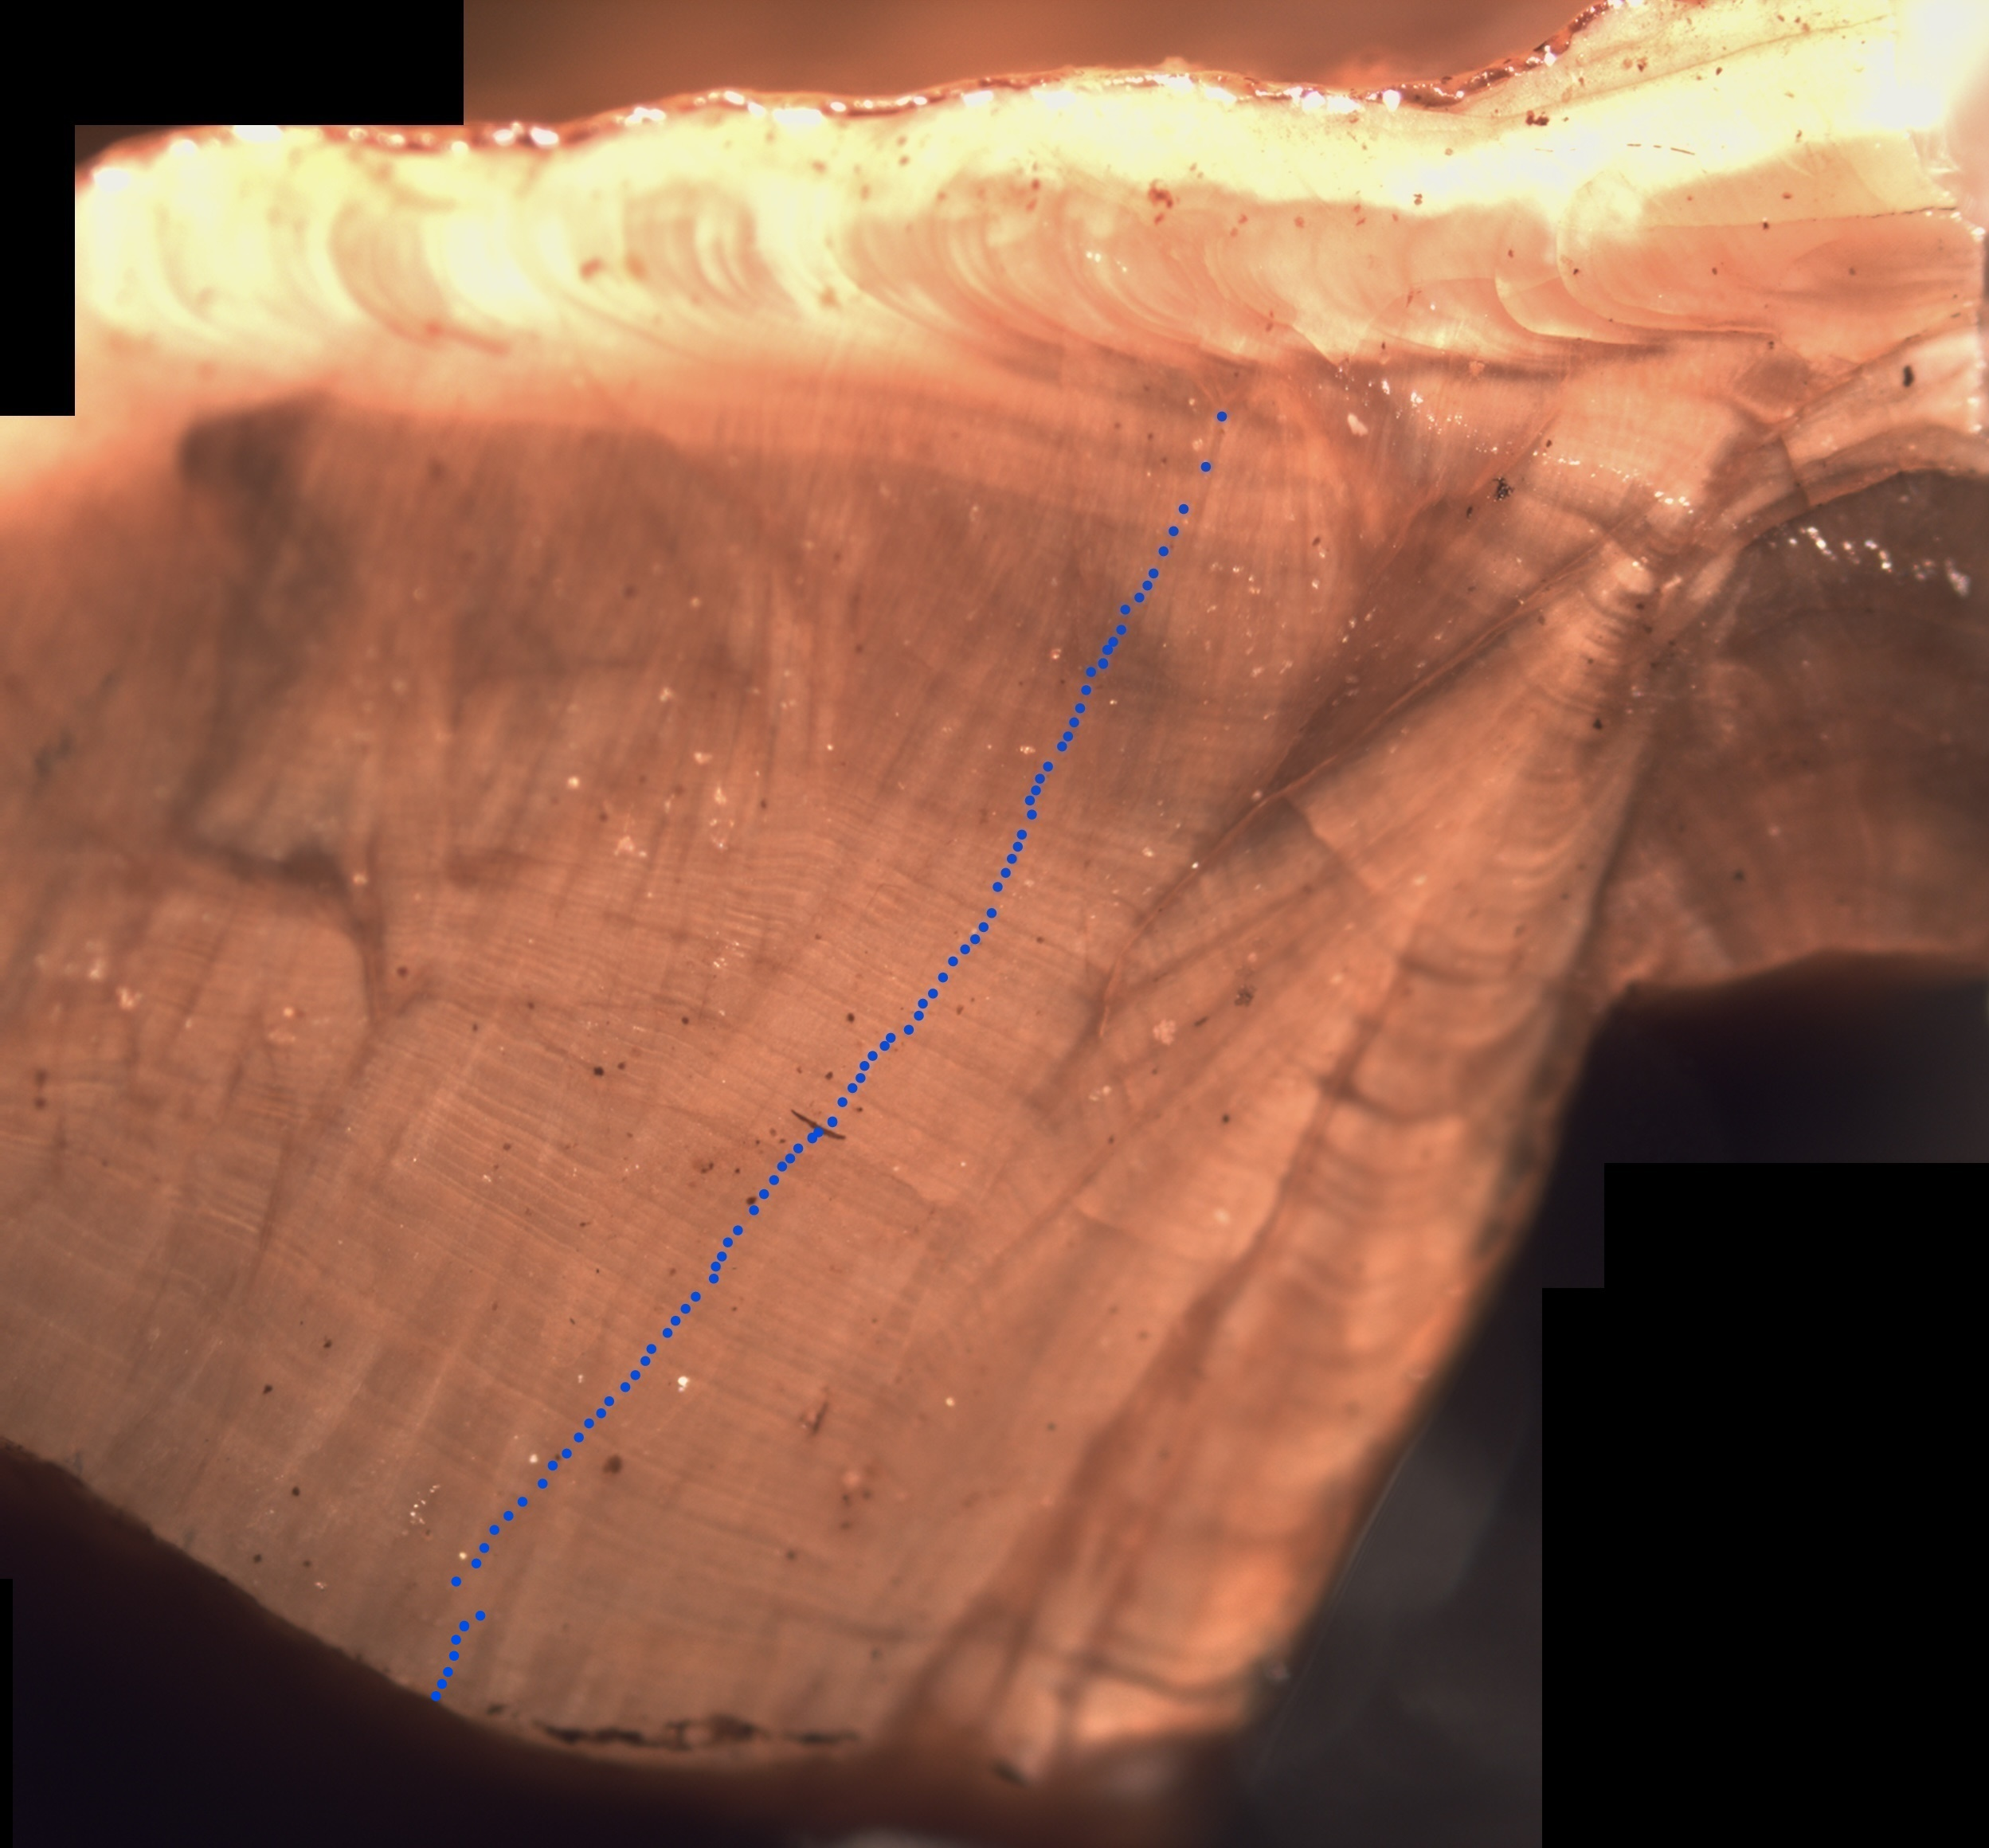
\includegraphics[width=1\textwidth,height=1\textheight]{C:/Stock_Assessments/VRML_Assessment_2021/GitHub/Vermilion_2021/doc/figures/oldfish.jpg}
\caption{Photograph of the \emph{oldest} aged fish used in the assessment with annuli marked by B. Kamikawa (NWFSC)..\label{fig:oldfish}}
\end{figure}

\begin{figure}
\centering
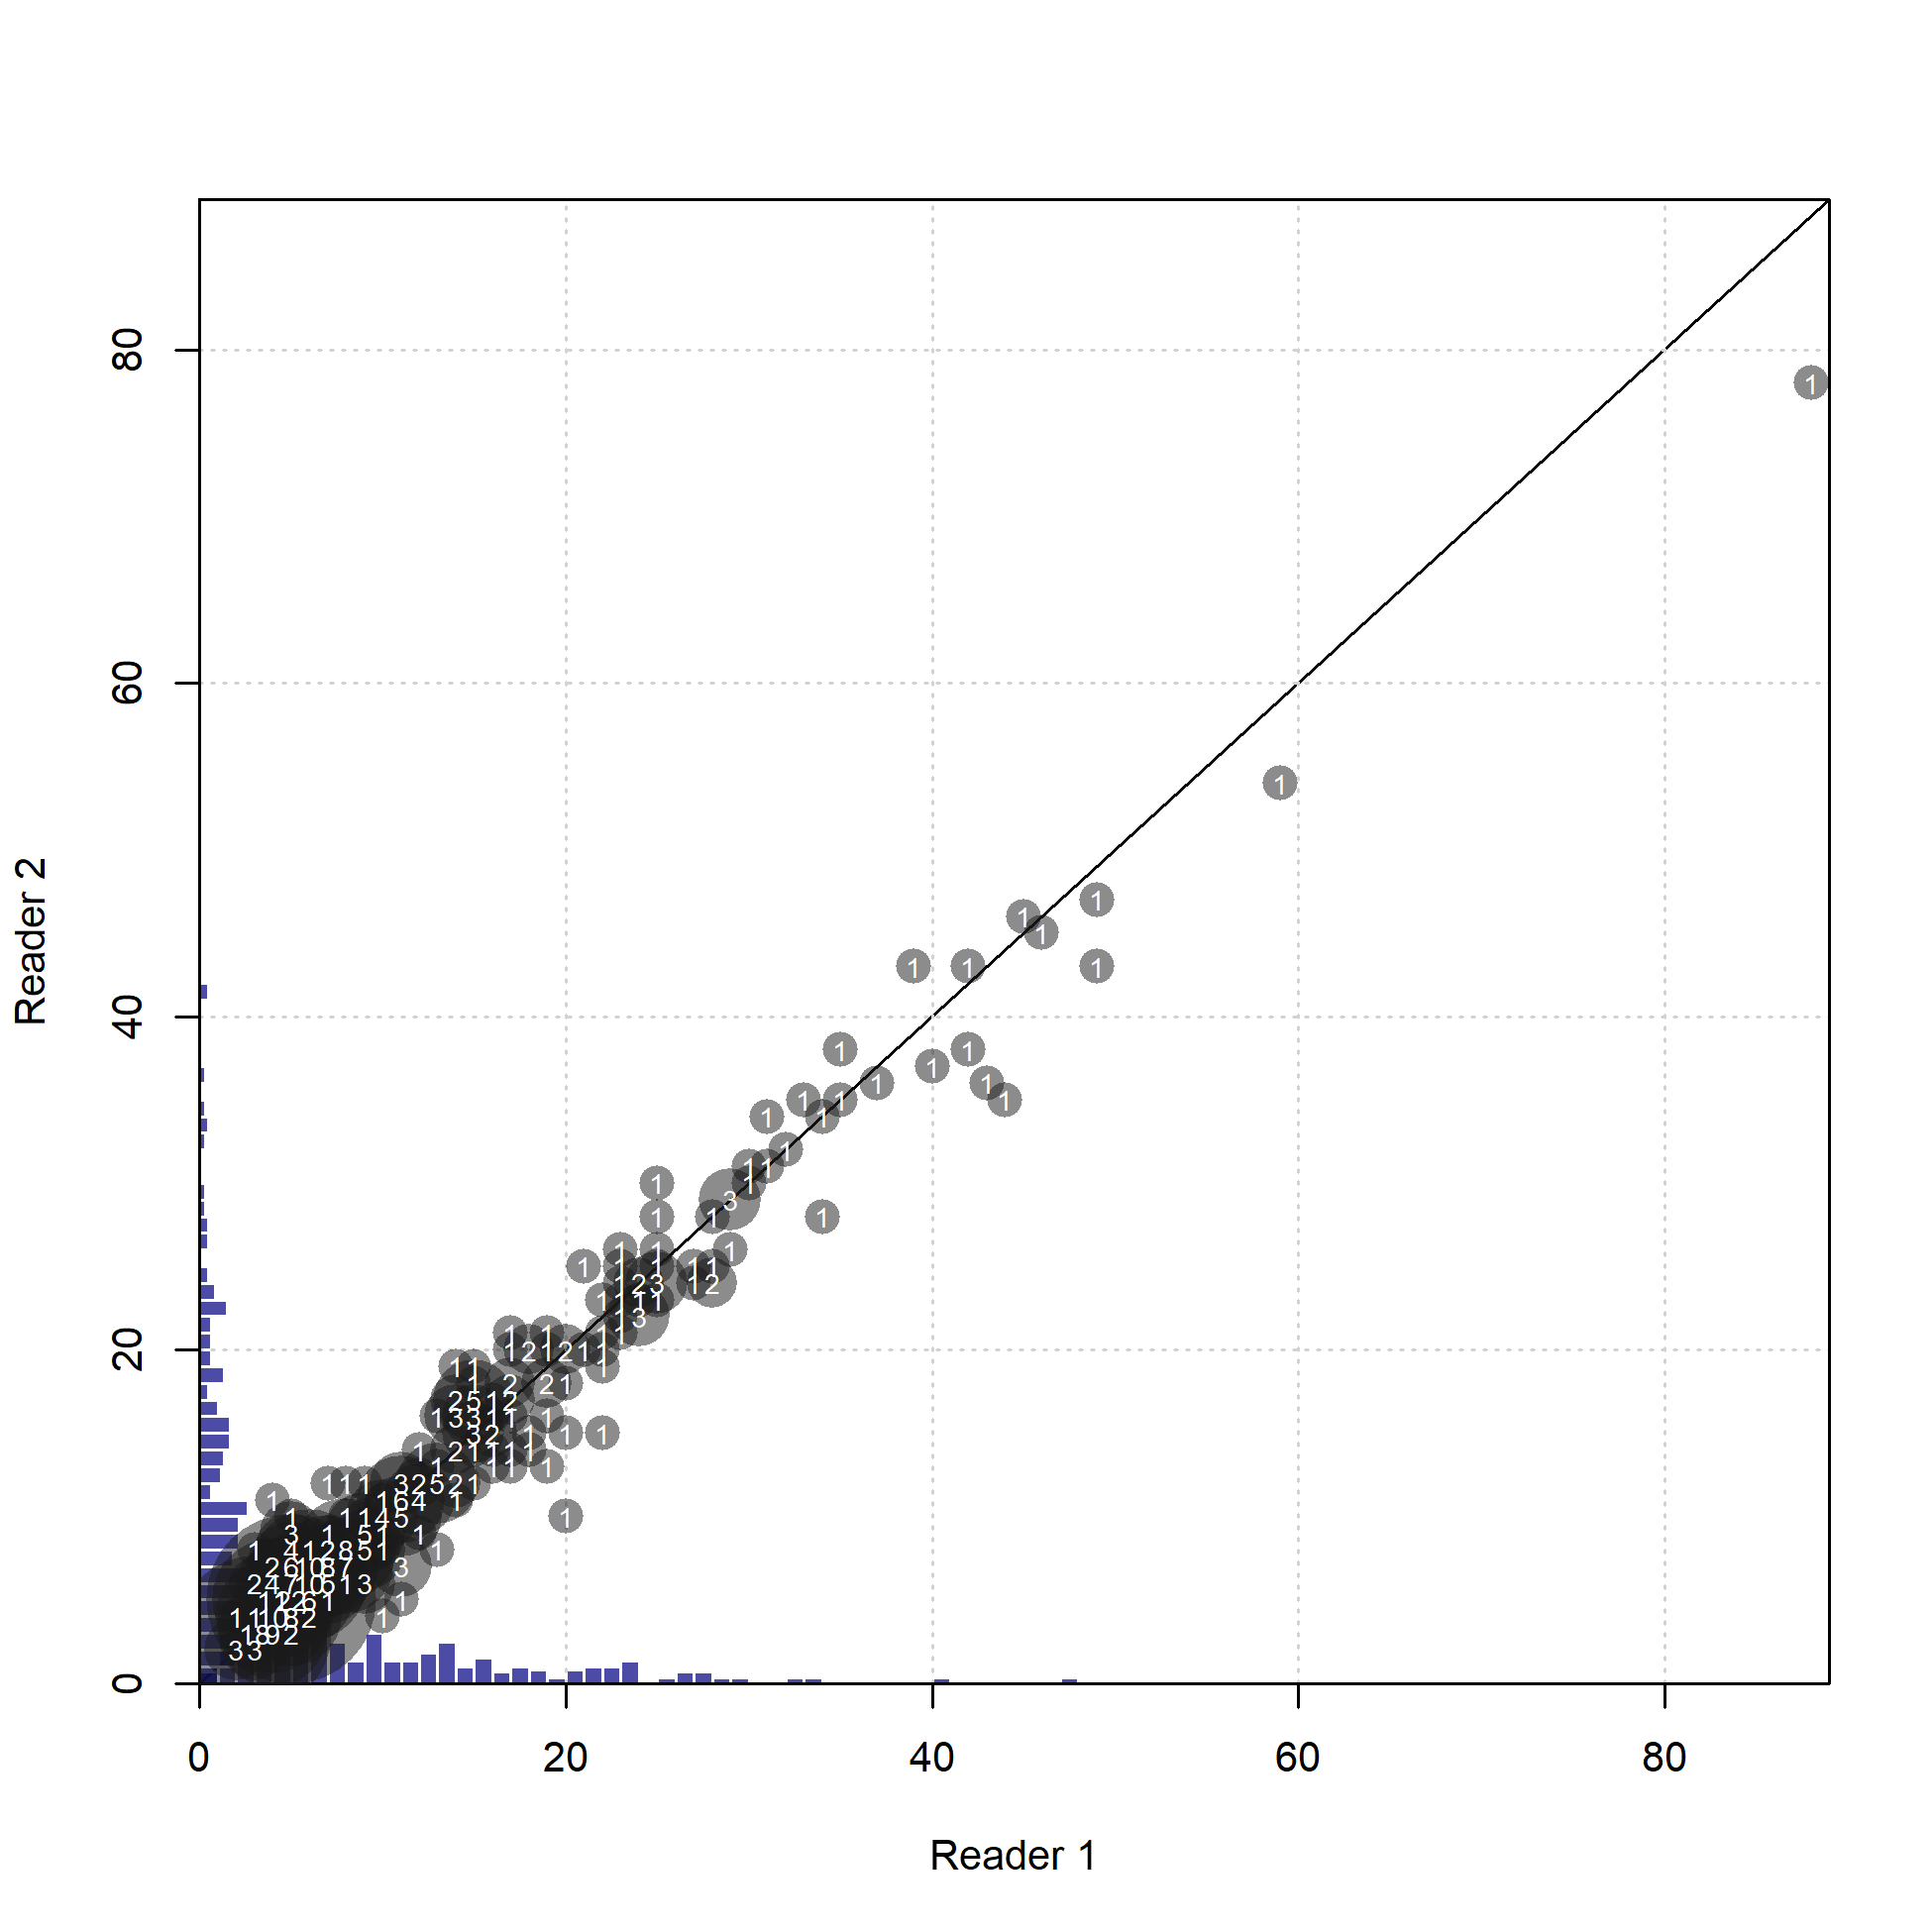
\includegraphics[width=1\textwidth,height=1\textheight]{C:/Stock_Assessments/VRML_Assessment_2021/GitHub/Vermilion_2021/doc/figures/Reader 1 vs Reader 2.png}
\caption{Aging precision between initial and blind double reads for vermilion. Numbers in the bubbles are the sample sizes of otoliths cross-read..\label{fig:reader1reader2}}
\end{figure}

\begin{figure}
\centering
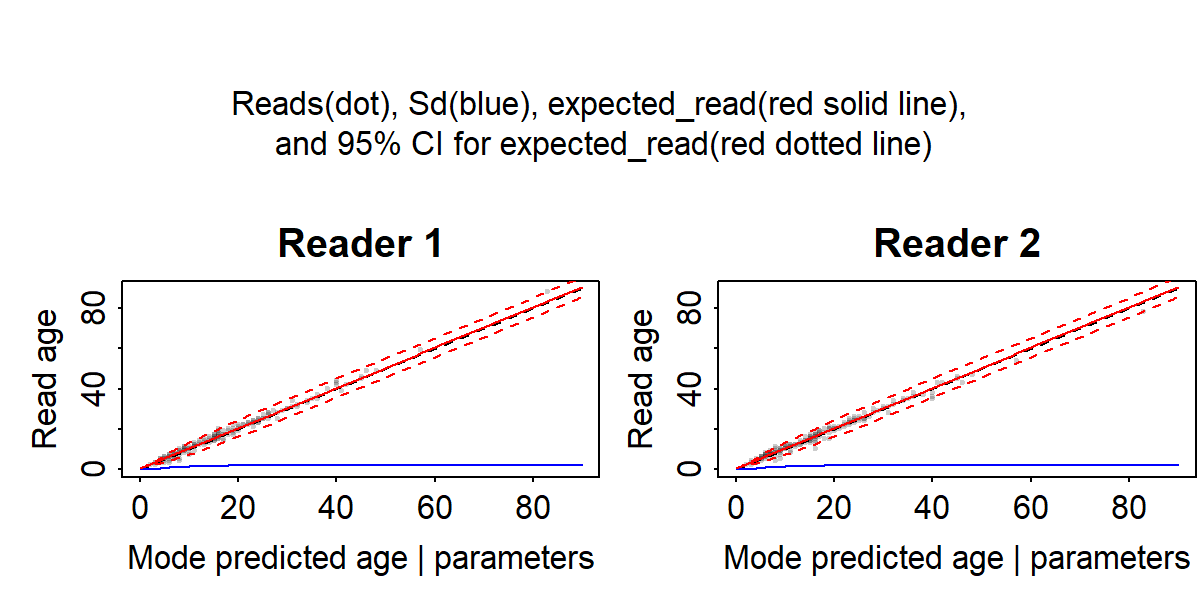
\includegraphics[width=1\textwidth,height=1\textheight]{C:/Stock_Assessments/VRML_Assessment_2021/GitHub/Vermilion_2021/doc/figures/True vs Reads (by reader).png}
\caption{True versus predicted age for two current age readers at the NWFSC from the ageing error software with unbiased reads for reader 1 and curvilinear bias for reader 1 and curvilinear standard deviation for both readers..\label{fig:truereads}}
\end{figure}

\begin{figure}
\centering
\includegraphics[width=1\textwidth,height=1\textheight]{C:/Stock_Assessments/VRML_Assessment_2021/Model_files/NCA/Verm21NoCA_060_time-varying_PC_and_PR/plots/sel01_multiple_fleets_length1.png}
\caption{Selectivity at length by fleet.\label{fig:selex}}
\end{figure}

\begin{figure}
\centering
\includegraphics[width=1\textwidth,height=1\textheight]{C:/Stock_Assessments/VRML_Assessment_2021/Model_files/NCA/Verm21NoCA_060_time-varying_PC_and_PR/plots/comp_lenfit_residsflt1mkt0.png}
\caption{Pearson residuals for the commercial hook-and-line fishery. Closed bubbles are positive residuals (observed \textgreater{} expected) and open bubbles are negative residuals (observed \textless{} expected).\label{fig:len-pearson-COM-HKL}}
\end{figure}

\begin{figure}
\centering
\includegraphics[width=1\textwidth,height=1\textheight]{C:/Stock_Assessments/VRML_Assessment_2021/Model_files/NCA/Verm21NoCA_060_time-varying_PC_and_PR/plots/comp_lenfit_data_weighting_TA1.8_COM_HKL.png}
\caption{Mean lengths for the commercial hook-and-line fishery with 95 percent confidence intervals based on current samples sizes.\label{fig:mean-len-fit-COM-HKL}}
\end{figure}

\begin{figure}
\centering
\includegraphics[width=1\textwidth,height=1\textheight]{C:/Stock_Assessments/VRML_Assessment_2021/Model_files/NCA/Verm21NoCA_060_time-varying_PC_and_PR/plots/comp_lenfit_residsflt2mkt0.png}
\caption{Pearson residuals for the commercial trawl fishery. Closed bubbles are positive residuals (observed \textgreater{} expected) and open bubbles are negative residuals (observed \textless{} expected).\label{fig:len-pearson-COM-TWL}}
\end{figure}

\begin{figure}
\centering
\includegraphics[width=1\textwidth,height=1\textheight]{C:/Stock_Assessments/VRML_Assessment_2021/Model_files/NCA/Verm21NoCA_060_time-varying_PC_and_PR/plots/comp_lenfit_data_weighting_TA1.8_COM_TWL.png}
\caption{Mean lengths for the commercial trawl fishery with 95 percent confidence intervals based on current samples sizes.\label{fig:mean-len-fit-COM-TWL}}
\end{figure}

\begin{figure}
\centering
\includegraphics[width=1\textwidth,height=1\textheight]{C:/Stock_Assessments/VRML_Assessment_2021/Model_files/NCA/Verm21NoCA_060_time-varying_PC_and_PR/plots/comp_lenfit_residsflt3mkt0.png}
\caption{Pearson residuals for the commercial net fishery. Closed bubbles are positive residuals (observed \textgreater{} expected) and open bubbles are negative residuals (observed \textless{} expected).\label{fig:len-pearson-COM-NET}}
\end{figure}

\begin{figure}
\centering
\includegraphics[width=1\textwidth,height=1\textheight]{C:/Stock_Assessments/VRML_Assessment_2021/Model_files/NCA/Verm21NoCA_060_time-varying_PC_and_PR/plots/comp_lenfit_data_weighting_TA1.8_COM_NET.png}
\caption{Mean lengths for the commercial net fishery with 95 percent confidence intervals based on current samples sizes.\label{fig:mean-len-fit-COM-NET}}
\end{figure}

\begin{figure}
\centering
\includegraphics[width=1\textwidth,height=1\textheight]{C:/Stock_Assessments/VRML_Assessment_2021/Model_files/NCA/Verm21NoCA_060_time-varying_PC_and_PR/plots/comp_lenfit_residsflt4mkt0_page2.png}
\caption{Pearson residuals for the recreational PC retained fishery. Closed bubbles are positive residuals (observed \textgreater{} expected) and open bubbles are negative residuals (observed \textless{} expected).\label{fig:len-pearson-REC-PC}}
\end{figure}

\begin{figure}
\centering
\includegraphics[width=1\textwidth,height=1\textheight]{C:/Stock_Assessments/VRML_Assessment_2021/Model_files/NCA/Verm21NoCA_060_time-varying_PC_and_PR/plots/comp_lenfit_data_weighting_TA1.8_REC_PC.png}
\caption{Mean lengths for the recreational PC retained fishery with 95 percent confidence intervals based on current samples sizes.\label{fig:mean-len-fit-REC-PC}}
\end{figure}

\begin{figure}
\centering
\includegraphics[width=1\textwidth,height=1\textheight]{C:/Stock_Assessments/VRML_Assessment_2021/Model_files/NCA/Verm21NoCA_060_time-varying_PC_and_PR/plots/comp_lenfit_residsflt5mkt0.png}
\caption{Pearson residuals for the recreational PC discard fishery. Closed bubbles are positive residuals (observed \textgreater{} expected) and open bubbles are negative residuals (observed \textless{} expected).\label{fig:len-pearson-REC-PC-DIS}}
\end{figure}

\begin{figure}
\centering
\includegraphics[width=1\textwidth,height=1\textheight]{C:/Stock_Assessments/VRML_Assessment_2021/Model_files/NCA/Verm21NoCA_060_time-varying_PC_and_PR/plots/comp_lenfit_data_weighting_TA1.8_REC_PC_DIS.png}
\caption{Mean lengths for the recreational PC discard fishery with 95 percent confidence intervals based on current samples sizes.\label{fig:mean-len-fit-REC-PC-DIS}}
\end{figure}

\begin{figure}
\centering
\includegraphics[width=1\textwidth,height=1\textheight]{C:/Stock_Assessments/VRML_Assessment_2021/Model_files/NCA/Verm21NoCA_060_time-varying_PC_and_PR/plots/comp_lenfit_residsflt6mkt0_page2.png}
\caption{Pearson residuals for the recreational PR retained fishery. Closed bubbles are positive residuals (observed \textgreater{} expected) and open bubbles are negative residuals (observed \textless{} expected).\label{fig:len-pearson-REC-PR}}
\end{figure}

\begin{figure}
\centering
\includegraphics[width=1\textwidth,height=1\textheight]{C:/Stock_Assessments/VRML_Assessment_2021/Model_files/NCA/Verm21NoCA_060_time-varying_PC_and_PR/plots/comp_lenfit_data_weighting_TA1.8_REC_PR.png}
\caption{Mean lengths for the recreational PR retained fishery with 95 percent confidence intervals based on current samples sizes.\label{fig:mean-len-fit-REC-PR}}
\end{figure}

\begin{figure}
\centering
\includegraphics[width=1\textwidth,height=1\textheight]{C:/Stock_Assessments/VRML_Assessment_2021/Model_files/NCA/Verm21NoCA_060_time-varying_PC_and_PR/plots/comp_lenfit_residsflt8mkt0.png}
\caption{Pearson residuals for the Deb Wilson-Vandenberg onboard survey. Closed bubbles are positive residuals (observed \textgreater{} expected) and open bubbles are negative residuals (observed \textless{} expected).\label{fig:len-pearson-DWV-ONBOARD}}
\end{figure}

\begin{figure}
\centering
\includegraphics[width=1\textwidth,height=1\textheight]{C:/Stock_Assessments/VRML_Assessment_2021/Model_files/NCA/Verm21NoCA_060_time-varying_PC_and_PR/plots/comp_lenfit_data_weighting_TA1.8_DWV_ONBOARD.png}
\caption{Mean lengths for the Deb Wilson-Vandenberg onboard survey with 95 percent confidence intervals based on current samples sizes.\label{fig:mean-len-fit-DWV-ONBOARD}}
\end{figure}

\begin{figure}
\centering
\includegraphics[width=1\textwidth,height=1\textheight]{C:/Stock_Assessments/VRML_Assessment_2021/Model_files/NCA/Verm21NoCA_060_time-varying_PC_and_PR/plots/comp_lenfit_residsflt9mkt0.png}
\caption{Pearson residuals for the West coast groundfish bottomfish trawl survey. Closed bubbles are positive residuals (observed \textgreater{} expected) and open bubbles are negative residuals (observed \textless{} expected).\label{fig:len-pearson-NWFSC-TWL}}
\end{figure}

\begin{figure}
\centering
\includegraphics[width=1\textwidth,height=1\textheight]{C:/Stock_Assessments/VRML_Assessment_2021/Model_files/NCA/Verm21NoCA_060_time-varying_PC_and_PR/plots/comp_lenfit_data_weighting_TA1.8_NWFSC_TWL.png}
\caption{Mean lengths for the West coast groundfish bottomfish trawl survey with 95 percent confidence intervals based on current samples sizes.\label{fig:mean-len-fit-NWFSC-TWL}}
\end{figure}

\begin{figure}
\centering
\includegraphics[width=1\textwidth,height=1\textheight]{C:/Stock_Assessments/VRML_Assessment_2021/Model_files/NCA/Verm21NoCA_060_time-varying_PC_and_PR/plots/comp_lenfit_residsflt11mkt0.png}
\caption{Pearson residuals for the Abrams thesis research survey. Closed bubbles are positive residuals (observed \textgreater{} expected) and open bubbles are negative residuals (observed \textless{} expected).\label{fig:len-pearson-ABRAMS-RESEARCH}}
\end{figure}

\begin{figure}
\centering
\includegraphics[width=1\textwidth,height=1\textheight]{C:/Stock_Assessments/VRML_Assessment_2021/Model_files/NCA/Verm21NoCA_060_time-varying_PC_and_PR/plots/comp_lenfit_data_weighting_TA1.8_ABRAMS_RESEARCH.png}
\caption{Mean lengths for the Abrams thesis research survey with 95 percent confidence intervals based on current samples sizes.\label{fig:mean-len-fit-ABRAMS-RESEARCH}}
\end{figure}

\begin{figure}
\centering
\includegraphics[width=1\textwidth,height=1\textheight]{C:/Stock_Assessments/VRML_Assessment_2021/Model_files/NCA/Verm21NoCA_060_time-varying_PC_and_PR/plots/comp_lenfit_residsflt12mkt0.png}
\caption{Pearson residuals for the SWFSC groundfish ecology survey. Closed bubbles are positive residuals (observed \textgreater{} expected) and open bubbles are negative residuals (observed \textless{} expected).\label{fig:len-pearson-SWFSC-GF-ECOL}}
\end{figure}

\begin{figure}
\centering
\includegraphics[width=1\textwidth,height=1\textheight]{C:/Stock_Assessments/VRML_Assessment_2021/Model_files/NCA/Verm21NoCA_060_time-varying_PC_and_PR/plots/comp_lenfit_data_weighting_TA1.8_SWFSC_GF_ECOL.png}
\caption{Mean lengths for the SWFSC groundfish ecology survey with 95 percent confidence intervals based on current samples sizes.\label{fig:mean-len-fit-SWFSC-GF-ECOL}}
\end{figure}

\begin{figure}
\centering
\includegraphics[width=1\textwidth,height=1\textheight]{C:/Stock_Assessments/VRML_Assessment_2021/Model_files/NCA/Verm21NoCA_060_time-varying_PC_and_PR/plots/comp_lenfit_residsflt13mkt0.png}
\caption{Pearson residuals for the California Collaborative Fisheries Research Project survey. Closed bubbles are positive residuals (observed \textgreater{} expected) and open bubbles are negative residuals (observed \textless{} expected).\label{fig:len-pearson-CCFRP}}
\end{figure}

\begin{figure}
\centering
\includegraphics[width=1\textwidth,height=1\textheight]{C:/Stock_Assessments/VRML_Assessment_2021/Model_files/NCA/Verm21NoCA_060_time-varying_PC_and_PR/plots/comp_lenfit_data_weighting_TA1.8_CCFRP.png}
\caption{Mean lengths for the California Collaborative Fisheries Research Project survey with 95 percent confidence intervals based on current samples sizes.\label{fig:mean-len-fit-CCFRP}}
\end{figure}

\begin{figure}
\centering
\includegraphics[width=1\textwidth,height=1\textheight]{C:/Stock_Assessments/VRML_Assessment_2021/Model_files/NCA/Verm21NoCA_060_time-varying_PC_and_PR/plots/ts7_Spawning_output_with_95_asymptotic_intervals_intervals.png}
\caption{Estimated time series of spawning output.\label{fig:ssb}}
\end{figure}

\begin{figure}
\centering
\includegraphics[width=1\textwidth,height=1\textheight]{C:/Stock_Assessments/VRML_Assessment_2021/Model_files/NCA/Verm21NoCA_060_time-varying_PC_and_PR/plots/ts1_Total_biomass_(mt).png}
\caption{Estimated time series of total biomass.\label{fig:tot-bio}}
\end{figure}

\begin{figure}
\centering
\includegraphics[width=1\textwidth,height=1\textheight]{C:/Stock_Assessments/VRML_Assessment_2021/Model_files/NCA/Verm21NoCA_060_time-varying_PC_and_PR/plots/ts9_Relative_spawning_output_intervals.png}
\caption{Estimated time series of relative spawning output.\label{fig:depl}}
\end{figure}

\begin{figure}
\centering
\includegraphics[width=1\textwidth,height=1\textheight]{C:/Stock_Assessments/VRML_Assessment_2021/Model_files/NCA/Verm21NoCA_060_time-varying_PC_and_PR/plots/ts11_Age-0_recruits_(1000s)_with_95_asymptotic_intervals.png}
\caption{Estimated time series of age-0 recruits (1000s).\label{fig:recruits}}
\end{figure}

\begin{figure}
\centering
\includegraphics[width=1\textwidth,height=1\textheight]{C:/Stock_Assessments/VRML_Assessment_2021/Model_files/NCA/Verm21NoCA_060_time-varying_PC_and_PR/plots/recdevs2_withbars.png}
\caption{Estimated time series of recruitment deviations.\label{fig:rec-devs}}
\end{figure}

\begin{figure}
\centering
\includegraphics[width=1\textwidth,height=1\textheight]{C:/Stock_Assessments/VRML_Assessment_2021/Model_files/NCA/Verm21NoCA_060_time-varying_PC_and_PR/plots/SR_curve.png}
\caption{Stock-recruit curve. Point colors indicate year, with warmer colors indicating earlier years and cooler colors in showing later years.\label{fig:bh-curve}}
\end{figure}

\begin{figure}
\centering
\includegraphics[width=1\textwidth,height=1\textheight]{C:/Stock_Assessments/VRML_Assessment_2021/Model_files/NCA/Verm21NoCA_060_time-varying_PC_and_PR/plots/SPR2_minusSPRseries.png}
\caption{Estimated 1 - relative spawning ratio (SPR) by year.\label{fig:1-spr}}
\end{figure}

\begin{figure}
\centering
\includegraphics[width=1\textwidth,height=1\textheight]{C:/Stock_Assessments/VRML_Assessment_2021/Model_files/NCA/Verm21NoCA_060_time-varying_PC_and_PR/plots/SPR4_phase.png}
\caption{Phase plot of the relative biomass (also referred to as fraction unfished) versus the SPR ratio where each point represents the biomass ratio at the start of the year and the relative fishing intensity in that same year. Lines through the final point show the 95 percent intervals based on the asymptotic uncertainty for each dimension. The shaded ellipse is a 95 percent region which accounts for the estimated correlations between the biomass ratio and SPR ratio.\label{fig:phase}}
\end{figure}

\begin{figure}
\centering
\includegraphics[width=1\textwidth,height=1\textheight]{C:/Stock_Assessments/VRML_Assessment_2021/Model_files/NCA/Verm21NoCA_060_time-varying_PC_and_PR/plots/yield2_yield_curve_with_refpoints.png}
\caption{Equilibrium yield curve for the base case model. Values are based on the 2020 fishery selectivity and with steepness fixed at 0.72.\label{fig:yield}}
\end{figure}

\newpage

\clearpage

\tagstructbegin{tag=H1}\tagmcbegin{tag=H1}

\hypertarget{appendix}{%
\section{Appendix}\label{appendix}}

\leavevmode\tagmcend\tagstructend

\tagstructbegin{tag=H3}\tagmcbegin{tag=H3}

\hypertarget{califronia-onboard-observer-survey-1999-2019}{%
\subsubsection{Califronia Onboard Observer Survey, 1999-2019}\label{califronia-onboard-observer-survey-1999-2019}}

\leavevmode\tagmcend\tagstructend

The state of California implemented a statewide onboard observer sampling program in 1999 {\tagstructbegin{tag=Reference}\tagmcbegin{tag=Reference}(M. H. Monk, Dick, and Pearson 2014)\leavevmode\tagmcend\tagstructend}. California Polytechnic State University (Cal Poly) has conducted an independent onboard sampling program as of 2003 for boats in Port San Luis and Morro Bay, and follows the protocols established in Reilly et al. {\tagstructbegin{tag=Reference}\tagmcbegin{tag=Reference}(1998)\leavevmode\tagmcend\tagstructend}.

During an onboard observer trip the sampler rides along on the CPFV and records location-specific catch and discard information to the species level for a subset of anglers onboard the vessel. The subset of observed anglers is usually a maximum of 15 people the observed anglers change during each fishing stop.\\
The catch cannot be linked to an individual, but rather to a specific fishing location. The sampler also records the starting and ending time, number of anglers observed, starting and ending depth, and measures discarded fish. The fine-scale catch and effort data allow us to better filter the data for indices to fishing stops within suitable habitat for vermilion. Cal Poly has modified protocols reflect sampling changes that CDFW has also adopted, e.g., observing fish as they are encountered instead of at the level of a fisher's bag. Therefore, the Cal Poly data area incorporated in the same index as the CDFW data from 1999-2019. The only difference is that Cal Poly measures the length of both retained and discarded fish.

Due to the COVID-19 pandemic, there are no onboard observer samples from either CDFW or Cal Poly in 2020.

\textbf{California CPFV CPUE Index: Data Preparation, Filtering, and Sample Sizes}

As described above the CDFW and Cal Poly onboard observer programs are identical in that the same protocols are followed. The only difference is that Cal Poly measures both retained and discarded fish from the observed anglers and CDFW measures only discarded fish from the observed anglers. CDFW measures retained fish as part of the angler interview at the bag and trip level. This index selectivity is mirrored to the recreational fleet in the stock assessment model, which represent only retained (dead) fish. Therefore, only retained fish were modeled in this index. The length from CDFW sampling are contained in the RecFIN database and indlucded in the length composition for the recreational fleet in the assessment model.

A number of filters are applied to these data. All of the Cal Poly data were QA/QC-ed once key-punched, whereas a number of errors remain in the data from CDFW. Data sheets from CDFW are not available prior to 2012 and staff constraints have also prevented a quality control review of the data.

Each drift was assigned to a reef (hard bottom). Hard bottom was extracted from the {\tagstructbegin{tag=Link}\tagmcbegin{tag=Link}\href{http://seafloor.otterlabs.org/index.html}{California Seafloor Mapping Project}\leavevmode\tagmcend\tagstructend}, with bathymetric data from state waters available at a 2 m resolution. Reefs were developed based on a number of factors described in the supplemental material (``Reef Delineation''). Depth restrictions in the recreational fishery were fairly consistent from 2004-2016. Starting in 2017, depth restrictions eased in districts north of Pt. Conception and the recreational fleet targeted these depths (Figure \ref{fig:fig-depthfished-cpfvonboard}. The deeper waters (40-50 fm) are outside of the mapped hard bottom habitat, but could be assigend to the larger areas considered as a factor in the index.

We retained 4481 drifts for index standardization, with 1706 drifts encountering vermilion (Table \ref{tab:tab-data-filter-cpfvonboard}).

Sample sizes by factors selected to model, excluding WAVE can be found in Tables \ref{tab:tab-region-cpfvonboard}, \ref{tab:tab-depth-cpfvonboard}, and \ref{tab:tab-year-cpfvonboard}.

\textbf{California CPFV CPUE Index: Model Selection, Fits, and Diagnostics}

We modeled retained catch per angler hour (CPUE; number of fish per angler hour) a Bayesian delta-GLM model. Indices with a year and area interaction were not considered in model selection; trends in the average CPUE by region were similar in the filtered data set (Figure \ref{fig:fig-areacpue-cpfvonboard}).

A Lognormal model was selected for the positive observation GLM by a {\tagstructbegin{tag=Formula}\tagmcbegin{tag=Formula}\(\Delta AIC\)\leavevmode\tagmcend\tagstructend} of 122.41 over a Gamma model and supported by Q-Q plots of the positive observations fit to both distributions (Figure \ref{fig:fig-dist-fits-cpfvonboard}). The delta-GLM method allows the linear predictors to differ between the binomial and positive models. Based on AIC values from maximum likelihood fits Table \ref{tab:tab-model-select-cpfvonboard}), a main effects model including YEAR and WAVE and DEPTH bin was fit for the binomial model and a main effects model including YEAR and WAVE and DEPTH bin was fit for the Lognormal model. Models were fit using the ``rstanarm'' R package (version 2.21.1). Posterior predictive checks of the Bayesian model fit for the binomial model and the positive model were all reasonable (Figures \ref{fig:fig-posterior-mean-cpfvonboard} and \ref{fig:fig-posterior-sd-cpfvonboard}). The binomial model generated data sets with the proportion zeros similar to the 62\% zeroes in the observed data (Figure \ref{fig:fig-propzero-cpfvonboard}). The predicted marginal effects from both the binomial and Lognormal models can be found in (Figures \ref{fig:fig-Dbin-marginal-cpfvonboard} and \ref{fig:fig-Dpos-marginal-cpfvonboard}). The final index (Table \ref{tab:tab-index-cpfvonboard}) represents a similar trend to the arithmetic mean of the annual CPUE (Figure \ref{fig:fig-cpue-cpfvonboard}).

\newpage

\begin{table}

\caption{\label{tab:tab-data-filter-cpfvonboard}Data filtering steps CA CPFV onboard survey index for vermilion in the northern model .}
\centering
\begin{tabular}[t]{>{\raggedright\arraybackslash}p{10em}>{\raggedright\arraybackslash}p{15em}c>{\centering\arraybackslash}p{5em}>{\centering\arraybackslash}p{5em}}
\toprule
Filter & Desciption & Trip & Positive Trips & Percent drifts retained\\
\midrule
\cellcolor{gray!6}{All} & \cellcolor{gray!6}{Download from SQL; identifiable errors filtered} & \cellcolor{gray!6}{6901} & \cellcolor{gray!6}{1755} & \cellcolor{gray!6}{25\%}\\
Fishery closed & Removed samples when target fish fishery closed & 5922 & 1736 & 29\%\\
\cellcolor{gray!6}{Ocean only} & \cellcolor{gray!6}{Removed samples from major bays} & \cellcolor{gray!6}{5780} & \cellcolor{gray!6}{1736} & \cellcolor{gray!6}{30\%}\\
Catch & Removed samples with zero catch of any species & 5335 & 1736 & 33\%\\
\cellcolor{gray!6}{Depth} & \cellcolor{gray!6}{Removed samples in less than max depth of species} & \cellcolor{gray!6}{5287} & \cellcolor{gray!6}{1736} & \cellcolor{gray!6}{33\%}\\
\addlinespace
Time fished & Removed upper two percent of time fished & 5180 & 1722 & 33\%\\
\cellcolor{gray!6}{Percent groundfish in samples} & \cellcolor{gray!6}{Removed samples with fewer groundfish than when the target observed} & \cellcolor{gray!6}{4481} & \cellcolor{gray!6}{1706} & \cellcolor{gray!6}{38\%}\\
\bottomrule
\end{tabular}
\end{table}

\begin{table}

\caption{\label{tab:tab-depth-cpfvonboard}Positive samples of vermilion in the northern model by depth (fm).}
\centering
\begin{tabular}[t]{lrrl}
\toprule
Year & Samples & Positive Samples & Percent Positive\\
\midrule
\cellcolor{gray!6}{(0,10]} & \cellcolor{gray!6}{40} & \cellcolor{gray!6}{346} & \cellcolor{gray!6}{12\%}\\
(10,15] & 139 & 559 & 25\%\\
\cellcolor{gray!6}{(15,20]} & \cellcolor{gray!6}{279} & \cellcolor{gray!6}{808} & \cellcolor{gray!6}{35\%}\\
(20,25] & 226 & 588 & 38\%\\
\cellcolor{gray!6}{(25,30]} & \cellcolor{gray!6}{219} & \cellcolor{gray!6}{601} & \cellcolor{gray!6}{36\%}\\
\addlinespace
(30,35] & 159 & 373 & 43\%\\
\cellcolor{gray!6}{(35,40]} & \cellcolor{gray!6}{216} & \cellcolor{gray!6}{450} & \cellcolor{gray!6}{48\%}\\
(40,65] & 428 & 756 & 57\%\\
\bottomrule
\end{tabular}
\end{table}

\FloatBarrier

\begin{table}

\caption{\label{tab:tab-region-cpfvonboard}Samples of vermilion in the northern model by subregion used in the index.}
\centering
\begin{tabular}[t]{lrrl}
\toprule
Year & Samples & Positive Samples & Percent Positive\\
\midrule
\cellcolor{gray!6}{CA/OR border to Santa Cruz (V1)} & \cellcolor{gray!6}{238} & \cellcolor{gray!6}{1213} & \cellcolor{gray!6}{20\%}\\
Moss Landing to Big Sur (V2) & 146 & 511 & 29\%\\
\cellcolor{gray!6}{San Luis Obsipso to Morro Bay (V3)} & \cellcolor{gray!6}{591} & \cellcolor{gray!6}{1044} & \cellcolor{gray!6}{57\%}\\
South Morro Bay to Point Conception (V4) & 643 & 1180 & 54\%\\
\cellcolor{gray!6}{Offshore (V5)} & \cellcolor{gray!6}{88} & \cellcolor{gray!6}{533} & \cellcolor{gray!6}{17\%}\\
\bottomrule
\end{tabular}
\end{table}

\begin{table}

\caption{\label{tab:tab-year-cpfvonboard}Samples of vermilion in the northern model by year.}
\centering
\begin{tabular}[t]{lrrl}
\toprule
Year & Samples & Positive Samples & Percent Positive\\
\midrule
\cellcolor{gray!6}{1999} & \cellcolor{gray!6}{13} & \cellcolor{gray!6}{60} & \cellcolor{gray!6}{22\%}\\
2000 & 6 & 38 & 16\%\\
\cellcolor{gray!6}{2001} & \cellcolor{gray!6}{11} & \cellcolor{gray!6}{71} & \cellcolor{gray!6}{15\%}\\
2002 & 17 & 60 & 28\%\\
\cellcolor{gray!6}{2003} & \cellcolor{gray!6}{117} & \cellcolor{gray!6}{276} & \cellcolor{gray!6}{42\%}\\
\addlinespace
2004 & 192 & 400 & 48\%\\
\cellcolor{gray!6}{2005} & \cellcolor{gray!6}{67} & \cellcolor{gray!6}{153} & \cellcolor{gray!6}{44\%}\\
2006 & 121 & 265 & 46\%\\
\cellcolor{gray!6}{2007} & \cellcolor{gray!6}{126} & \cellcolor{gray!6}{268} & \cellcolor{gray!6}{47\%}\\
2008 & 47 & 155 & 30\%\\
\addlinespace
\cellcolor{gray!6}{2009} & \cellcolor{gray!6}{54} & \cellcolor{gray!6}{198} & \cellcolor{gray!6}{27\%}\\
2010 & 79 & 193 & 41\%\\
\cellcolor{gray!6}{2011} & \cellcolor{gray!6}{62} & \cellcolor{gray!6}{182} & \cellcolor{gray!6}{34\%}\\
2012 & 66 & 220 & 30\%\\
\cellcolor{gray!6}{2013} & \cellcolor{gray!6}{29} & \cellcolor{gray!6}{160} & \cellcolor{gray!6}{18\%}\\
\addlinespace
2014 & 47 & 221 & 21\%\\
\cellcolor{gray!6}{2015} & \cellcolor{gray!6}{75} & \cellcolor{gray!6}{219} & \cellcolor{gray!6}{34\%}\\
2016 & 79 & 321 & 25\%\\
\cellcolor{gray!6}{2017} & \cellcolor{gray!6}{226} & \cellcolor{gray!6}{426} & \cellcolor{gray!6}{53\%}\\
2018 & 146 & 295 & 49\%\\
\addlinespace
\cellcolor{gray!6}{2019} & \cellcolor{gray!6}{126} & \cellcolor{gray!6}{300} & \cellcolor{gray!6}{42\%}\\
\bottomrule
\end{tabular}
\end{table}

\FloatBarrier

\begin{table}

\caption{\label{tab:tab-model-select-cpfvonboard}Model selection for the CA CPFV onboard survey index for vermilion in the northern model .}
\centering
\begin{tabular}[t]{lrr}
\toprule
Model & Binomial $\Delta$AIC & Lognormal $\Delta$AIC\\
\midrule
\cellcolor{gray!6}{1} & \cellcolor{gray!6}{797.52} & \cellcolor{gray!6}{436.25}\\
YEAR + SubRegion & 129.05 & 60.03\\
\cellcolor{gray!6}{YEAR + SubRegion + WAVE} & \cellcolor{gray!6}{120.54} & \cellcolor{gray!6}{58.72}\\
YEAR + SubRegion + WAVE + DEPTH bin & 0.00 & 0.00\\
\cellcolor{gray!6}{YEAR + WAVE + DEPTH bin} & \cellcolor{gray!6}{285.69} & \cellcolor{gray!6}{66.16}\\
\addlinespace
YEAR + DEPTH bin & 316.83 & 74.00\\
\cellcolor{gray!6}{YEAR + SubRegion + DEPTH bin} & \cellcolor{gray!6}{10.87} & \cellcolor{gray!6}{6.06}\\
\bottomrule
\end{tabular}
\end{table}

\FloatBarrier

\begin{table}

\caption{\label{tab:tab-index-cpfvonboard}Standardized index for the CA CPFV onboard survey index with log-scale standard errors and 95% highest
       posterior density (HPD) intervals for vermilion in the northern model .}
\centering
\begin{tabular}[t]{rrrrr}
\toprule
Year & Mean & logSE & lower HPD & upper HPD\\
\midrule
\cellcolor{gray!6}{1999} & \cellcolor{gray!6}{0.02} & \cellcolor{gray!6}{0.53} & \cellcolor{gray!6}{0.01} & \cellcolor{gray!6}{0.05}\\
2000 & 0.02 & 0.65 & 0.00 & 0.04\\
\cellcolor{gray!6}{2001} & \cellcolor{gray!6}{0.01} & \cellcolor{gray!6}{0.53} & \cellcolor{gray!6}{0.00} & \cellcolor{gray!6}{0.02}\\
2002 & 0.02 & 0.42 & 0.01 & 0.05\\
\cellcolor{gray!6}{2003} & \cellcolor{gray!6}{0.05} & \cellcolor{gray!6}{0.33} & \cellcolor{gray!6}{0.02} & \cellcolor{gray!6}{0.09}\\
\addlinespace
2004 & 0.07 & 0.28 & 0.04 & 0.11\\
\cellcolor{gray!6}{2005} & \cellcolor{gray!6}{0.04} & \cellcolor{gray!6}{0.38} & \cellcolor{gray!6}{0.02} & \cellcolor{gray!6}{0.08}\\
2006 & 0.05 & 0.36 & 0.02 & 0.09\\
\cellcolor{gray!6}{2007} & \cellcolor{gray!6}{0.06} & \cellcolor{gray!6}{0.35} & \cellcolor{gray!6}{0.03} & \cellcolor{gray!6}{0.11}\\
2008 & 0.03 & 0.38 & 0.01 & 0.05\\
\addlinespace
\cellcolor{gray!6}{2009} & \cellcolor{gray!6}{0.04} & \cellcolor{gray!6}{0.37} & \cellcolor{gray!6}{0.02} & \cellcolor{gray!6}{0.07}\\
2010 & 0.05 & 0.37 & 0.02 & 0.09\\
\cellcolor{gray!6}{2011} & \cellcolor{gray!6}{0.04} & \cellcolor{gray!6}{0.37} & \cellcolor{gray!6}{0.02} & \cellcolor{gray!6}{0.08}\\
2012 & 0.03 & 0.38 & 0.01 & 0.06\\
\cellcolor{gray!6}{2013} & \cellcolor{gray!6}{0.02} & \cellcolor{gray!6}{0.42} & \cellcolor{gray!6}{0.01} & \cellcolor{gray!6}{0.04}\\
\addlinespace
2014 & 0.02 & 0.38 & 0.01 & 0.04\\
\cellcolor{gray!6}{2015} & \cellcolor{gray!6}{0.04} & \cellcolor{gray!6}{0.37} & \cellcolor{gray!6}{0.02} & \cellcolor{gray!6}{0.07}\\
2016 & 0.03 & 0.37 & 0.01 & 0.06\\
\cellcolor{gray!6}{2017} & \cellcolor{gray!6}{0.04} & \cellcolor{gray!6}{0.36} & \cellcolor{gray!6}{0.02} & \cellcolor{gray!6}{0.08}\\
2018 & 0.05 & 0.37 & 0.02 & 0.09\\
\addlinespace
\cellcolor{gray!6}{2019} & \cellcolor{gray!6}{0.04} & \cellcolor{gray!6}{0.37} & \cellcolor{gray!6}{0.02} & \cellcolor{gray!6}{0.08}\\
\bottomrule
\end{tabular}
\end{table}

\FloatBarrier

\begin{figure}
\centering
\includegraphics{C:/Stock_Assessments/VRML_Assessment_2021/GitHub/Vermilion_2021/doc/indices/vermilion_CA_CPFV_onboard_writeup_NCA_files/figure-latex/fig-dist-fits-cpfvonboard-1.pdf}
\caption{\label{fig:fig-dist-fits-cpfvonboard}Q-Q plot (top) of the positive observations lognormal gamma distributions and fitted values vs residuals for the Lognormal model (bottom).}
\end{figure}

\begin{figure}
\centering
\includegraphics{C:/Stock_Assessments/VRML_Assessment_2021/GitHub/Vermilion_2021/doc/indices/vermilion_CA_CPFV_onboard_writeup_NCA_files/figure-latex/fig-depthfished-cpfvonboard-1.pdf}
\caption{\label{fig:fig-depthfished-cpfvonboard}Boxplots of depths fished by year in the filtered data.}
\end{figure}

\begin{figure}
\centering
\includegraphics{C:/Stock_Assessments/VRML_Assessment_2021/GitHub/Vermilion_2021/doc/indices/vermilion_CA_CPFV_onboard_writeup_NCA_files/figure-latex/fig-areacpue-cpfvonboard-1.pdf}
\caption{\label{fig:fig-areacpue-cpfvonboard}Arithmetic mean of CPUE by region for vermilion from the filtered data. The areas used are in the text.}
\end{figure}

\begin{figure}
\centering
\includegraphics{C:/Stock_Assessments/VRML_Assessment_2021/GitHub/Vermilion_2021/doc/indices/vermilion_CA_CPFV_onboard_writeup_NCA_files/figure-latex/fig-propzero-cpfvonboard-1.pdf}
\caption{\label{fig:fig-propzero-cpfvonboard}Posterior predictive distribution of the proportion of zero observations in replicate data sets generated by the delta model with a vertical line representing the observed average.}
\end{figure}

\begin{figure}
\centering
\includegraphics{C:/Stock_Assessments/VRML_Assessment_2021/GitHub/Vermilion_2021/doc/indices/vermilion_CA_CPFV_onboard_writeup_NCA_files/figure-latex/fig-posterior-mean-cpfvonboard-1.pdf}
\caption{\label{fig:fig-posterior-mean-cpfvonboard}Posterior predictive draws of the mean by year with a vertical line representing the observed average.}
\end{figure}

\begin{figure}
\centering
\includegraphics{C:/Stock_Assessments/VRML_Assessment_2021/GitHub/Vermilion_2021/doc/indices/vermilion_CA_CPFV_onboard_writeup_NCA_files/figure-latex/fig-posterior-sd-cpfvonboard-1.pdf}
\caption{\label{fig:fig-posterior-sd-cpfvonboard}Posterior predictive draws of the standard deviation by year with a vertical line representing the observed average.}
\end{figure}

\begin{figure}
\centering
\includegraphics{C:/Stock_Assessments/VRML_Assessment_2021/GitHub/Vermilion_2021/doc/indices/vermilion_CA_CPFV_onboard_writeup_NCA_files/figure-latex/fig-cpue-cpfvonboard-1.pdf}
\caption{\label{fig:fig-cpue-cpfvonboard}Standardized index and arithmetic mean of the CPUE from the filtered data. Each timeseries is scaled to its respective means.}
\end{figure}

\begin{figure}
\centering
\includegraphics{C:/Stock_Assessments/VRML_Assessment_2021/GitHub/Vermilion_2021/doc/indices/vermilion_CA_CPFV_onboard_writeup_NCA_files/figure-latex/fig-Dbin-marginal-cpfvonboard-1.pdf}
\caption{\label{fig:fig-Dbin-marginal-cpfvonboard}Binomial marginal effects from the final model}
\end{figure}

\begin{figure}
\centering
\includegraphics{C:/Stock_Assessments/VRML_Assessment_2021/GitHub/Vermilion_2021/doc/indices/vermilion_CA_CPFV_onboard_writeup_NCA_files/figure-latex/fig-Dpos-marginal-cpfvonboard-1.pdf}
\caption{\label{fig:fig-Dpos-marginal-cpfvonboard}Positive model marginal effects from the final model.}
\end{figure}

\tagstructbegin{tag=H3}\tagmcbegin{tag=H3}

\hypertarget{california-collaborative-fisheries-research-project-index}{%
\subsubsection{California Collaborative Fisheries Research Project Index}\label{california-collaborative-fisheries-research-project-index}}

\leavevmode\tagmcend\tagstructend

The California Collaborative Fisheries Research Project, {\tagstructbegin{tag=Link}\tagmcbegin{tag=Link}\href{https://www.mlml.calstate.edu/ccfrp/}{CCFRP}\leavevmode\tagmcend\tagstructend}, is a fishery-independent hook-and-line survey designed to monitor nearshore fish populations at a series of sampling locations both inside and adjacent to MPAs along the central California coast {\tagstructbegin{tag=Reference}\tagmcbegin{tag=Reference}(Wendt and Starr 2009; Starr et al. 2015)\leavevmode\tagmcend\tagstructend}. The CCFRP survey began in 2007 and was originally designed as a statewide program in collaboration with NMFS scientists and fishermen. From 2007-2016 the CCFRP project was focused on the central California coast, and has monitored four MPAs consistently. In 2017, the program was expanded coastwide within California. The index of abundance was developed from the four MPAs sampled consistently (Año Nuevo and Point Lobos by Moss Landing Marine Labs; Point Buchon and Piedras Blancas by Cal Poly).

The survey design for CCFRP consists a number 500 x 500 m cells both within and outside each MPA. On any given survey day site cells are randomly selected within a stratum (MPA and/or reference cells). CPFVs are chartered for the survey and the fishing captain is allowed to search within the cell for a fishing location. During a sampling event, each cell is fished for a total of 30-45 minutes by volunteer anglers. Each fish encountered is recorded, measured, and can be linked back to a particular angler, and released (or descended to depth). Starting in 2017, a subset of fish have been retained to collect otoliths and fin clips that provide needed biological information for nearshore species. For the index of abundance, CPUE was modeled at the level of the drift, similar to the fishery-dependent onboard observer survey described above.

\emph{CCFRP Index: Data Preparation, Filtering, and Sample Sizes}

The CCFRP data are quality controlled at the time they are key punched and little filtering was needed for the index. Cells not consistently sampled over time were excluded as well as cells that never encountered vermilion. CCFRP samples shallower depths to avoid barotrauma-induced mortality. We retained 6532 drifts for index standardization, with 2250 drifts encountering vermilion.

\emph{CCFRP Index: Model Selection, Fits, and Diagnostics}

Sample sizes by factors selected to model, excluding WAVE can be found in Tables \ref{tab:tab-region-ccfrp} and \ref{tab:tab-year-ccfrp}. We modeled retained catch per angler hour (CPUE; number of fish per angler hour) a Bayesian delta-GLM model. Indices with a year and area interaction were not considered in model selection; trends in the average CPUE by region were similar in the filtered data set (Figure \ref{fig:fig-areacpue-ccfrp}). Plots of the arithmetic mean by inside (MPA) and outside (REF) MPAs over time is in Figure \ref{fig:fig-sitecpue-ccfrp}.

A Lognormal model was selected for the positive observation GLM by a {\tagstructbegin{tag=Formula}\tagmcbegin{tag=Formula}\(\Delta AIC\)\leavevmode\tagmcend\tagstructend} of 362.81 over a Gamma model and supported by Q-Q plots of the positive observations fit to both distributions (Figure \ref{fig:fig-dist-fits-ccfrp}). The delta-GLM method allows the linear predictors to differ between the binomial and positive models. Based on AIC values from maximum likelihood fits Table \ref{tab:tab-model-select-ccfrp}), a main effects model including YEAR and SITE and DEPTH bin was fit for the binomial model and a main effects model including YEAR and SITE and DEPTH bin was fit for the Lognormal model. Models were fit using the ``rstanarm'' R package (version 2.21.1). Posterior predictive checks of the Bayesian model fit for the binomial model and the positive model were all reasonable (Figures \ref{fig:fig-posterior-mean-ccfrp} and \ref{fig:fig-posterior-sd-ccfrp}). The binomial model generated data sets with the proportion zeros similar to the 66\% zeroes in the observed data (Figure \ref{fig:fig-propzero-ccfrp}). The predicted marginal effects from both the binomial and Lognormal models can be found in (Figures \ref{fig:fig-Dbin-marginal-ccfrp} and \ref{fig:fig-Dpos-marginal-ccfrp}). The final index (Table \ref{tab:tab-index-ccfrp}) represents a similar trend to the arithmetic mean of the annual CPUE (Figure \ref{fig:fig-cpue-ccfrp}).

\newpage

\begin{table}

\caption{\label{tab:tab-region-ccfrp}Samples of vermilion in the northern model by subregion used in the index.}
\centering
\begin{tabular}[t]{lrrl}
\toprule
Year & Samples & Positive Samples & Percent Positive\\
\midrule
\cellcolor{gray!6}{South Cape Mendocino} & \cellcolor{gray!6}{84} & \cellcolor{gray!6}{277} & \cellcolor{gray!6}{30\%}\\
Ten Mile & 45 & 224 & 20\%\\
\cellcolor{gray!6}{Stewarts Point} & \cellcolor{gray!6}{111} & \cellcolor{gray!6}{279} & \cellcolor{gray!6}{40\%}\\
Bodega Head & 43 & 214 & 20\%\\
\cellcolor{gray!6}{Ano Nuevo} & \cellcolor{gray!6}{484} & \cellcolor{gray!6}{1879} & \cellcolor{gray!6}{26\%}\\
\addlinespace
Point Lobos & 375 & 1369 & 27\%\\
\cellcolor{gray!6}{Piedras Blancas} & \cellcolor{gray!6}{614} & \cellcolor{gray!6}{966} & \cellcolor{gray!6}{64\%}\\
Point Buchon & 494 & 1324 & 37\%\\
\bottomrule
\end{tabular}
\end{table}

\begin{table}

\caption{\label{tab:tab-depth-ccfrp}Positive samples of vermilion in the northern model by depth (fm).}
\centering
\begin{tabular}[t]{lrrl}
\toprule
Year & Samples & Positive Samples & Percent Positive\\
\midrule
\cellcolor{gray!6}{(0,10]} & \cellcolor{gray!6}{385} & \cellcolor{gray!6}{1712} & \cellcolor{gray!6}{22\%}\\
(10,15] & 1019 & 2780 & 37\%\\
\cellcolor{gray!6}{(15,20]} & \cellcolor{gray!6}{741} & \cellcolor{gray!6}{1713} & \cellcolor{gray!6}{43\%}\\
(20,30] & 105 & 327 & 32\%\\
\bottomrule
\end{tabular}
\end{table}

\begin{table}

\caption{\label{tab:tab-year-ccfrp}Samples of vermilion in the northern model by year.}
\centering
\begin{tabular}[t]{lrrl}
\toprule
Year & Samples & Positive Samples & Percent Positive\\
\midrule
\cellcolor{gray!6}{2007} & \cellcolor{gray!6}{96} & \cellcolor{gray!6}{552} & \cellcolor{gray!6}{17\%}\\
2008 & 123 & 564 & 22\%\\
\cellcolor{gray!6}{2009} & \cellcolor{gray!6}{115} & \cellcolor{gray!6}{371} & \cellcolor{gray!6}{31\%}\\
2010 & 171 & 427 & 40\%\\
\cellcolor{gray!6}{2011} & \cellcolor{gray!6}{142} & \cellcolor{gray!6}{374} & \cellcolor{gray!6}{38\%}\\
\addlinespace
2012 & 163 & 397 & 41\%\\
\cellcolor{gray!6}{2013} & \cellcolor{gray!6}{110} & \cellcolor{gray!6}{430} & \cellcolor{gray!6}{26\%}\\
2014 & 162 & 449 & 36\%\\
\cellcolor{gray!6}{2015} & \cellcolor{gray!6}{98} & \cellcolor{gray!6}{224} & \cellcolor{gray!6}{44\%}\\
2016 & 174 & 429 & 41\%\\
\addlinespace
\cellcolor{gray!6}{2017} & \cellcolor{gray!6}{190} & \cellcolor{gray!6}{516} & \cellcolor{gray!6}{37\%}\\
2018 & 228 & 582 & 39\%\\
\cellcolor{gray!6}{2019} & \cellcolor{gray!6}{260} & \cellcolor{gray!6}{622} & \cellcolor{gray!6}{42\%}\\
2020 & 218 & 595 & 37\%\\
\bottomrule
\end{tabular}
\end{table}

\FloatBarrier

\begin{table}

\caption{\label{tab:tab-model-select-ccfrp}Model selection for the CCFRP survey index for vermilion in the northern model .}
\centering
\begin{tabular}[t]{lrr}
\toprule
Model & Binomial $\Delta$AIC & Lognormal $\Delta$AIC\\
\midrule
\cellcolor{gray!6}{1} & \cellcolor{gray!6}{1071.49} & \cellcolor{gray!6}{485.95}\\
YEAR + AREA & 423.29 & 163.14\\
\cellcolor{gray!6}{YEAR + AREA + SITE} & \cellcolor{gray!6}{79.34} & \cellcolor{gray!6}{40.23}\\
YEAR + AREA + SITE + DEPTH bin & 0.00 & 0.00\\
\cellcolor{gray!6}{YEAR + SITE + DEPTH bin} & \cellcolor{gray!6}{470.88} & \cellcolor{gray!6}{88.31}\\
\addlinespace
YEAR + DEPTH bin & 727.53 & 185.13\\
\cellcolor{gray!6}{YEAR + AREA + DEPTH bin} & \cellcolor{gray!6}{292.96} & \cellcolor{gray!6}{113.84}\\
\bottomrule
\end{tabular}
\end{table}

\FloatBarrier

\begin{table}

\caption{\label{tab:tab-index-ccfrp}Standardized index for the CCFRP survey index with log-scale standard errors and 95% highest
       posterior density (HPD) intervals for vermilion in the northern model .}
\centering
\begin{tabular}[t]{rrrrr}
\toprule
Year & Mean & logSE & lower HPD & upper HPD\\
\midrule
\cellcolor{gray!6}{2007} & \cellcolor{gray!6}{0.12} & \cellcolor{gray!6}{0.22} & \cellcolor{gray!6}{0.08} & \cellcolor{gray!6}{0.19}\\
2008 & 0.10 & 0.21 & 0.06 & 0.14\\
\cellcolor{gray!6}{2009} & \cellcolor{gray!6}{0.17} & \cellcolor{gray!6}{0.21} & \cellcolor{gray!6}{0.11} & \cellcolor{gray!6}{0.24}\\
2010 & 0.24 & 0.19 & 0.16 & 0.33\\
\cellcolor{gray!6}{2011} & \cellcolor{gray!6}{0.19} & \cellcolor{gray!6}{0.20} & \cellcolor{gray!6}{0.13} & \cellcolor{gray!6}{0.28}\\
\addlinespace
2012 & 0.20 & 0.19 & 0.13 & 0.28\\
\cellcolor{gray!6}{2013} & \cellcolor{gray!6}{0.10} & \cellcolor{gray!6}{0.22} & \cellcolor{gray!6}{0.06} & \cellcolor{gray!6}{0.15}\\
2014 & 0.18 & 0.19 & 0.12 & 0.26\\
\cellcolor{gray!6}{2015} & \cellcolor{gray!6}{0.26} & \cellcolor{gray!6}{0.20} & \cellcolor{gray!6}{0.17} & \cellcolor{gray!6}{0.38}\\
2016 & 0.19 & 0.19 & 0.13 & 0.28\\
\addlinespace
\cellcolor{gray!6}{2017} & \cellcolor{gray!6}{0.22} & \cellcolor{gray!6}{0.17} & \cellcolor{gray!6}{0.16} & \cellcolor{gray!6}{0.30}\\
2018 & 0.31 & 0.16 & 0.22 & 0.42\\
\cellcolor{gray!6}{2019} & \cellcolor{gray!6}{0.36} & \cellcolor{gray!6}{0.16} & \cellcolor{gray!6}{0.26} & \cellcolor{gray!6}{0.48}\\
2020 & 0.48 & 0.16 & 0.34 & 0.65\\
\bottomrule
\end{tabular}
\end{table}

\FloatBarrier

\begin{figure}
\centering
\includegraphics{C:/Stock_Assessments/VRML_Assessment_2021/GitHub/Vermilion_2021/doc/indices/vermilion_CCFRP_writeup_NCA_files/figure-latex/fig-dist-fits-ccfrp-1.pdf}
\caption{\label{fig:fig-dist-fits-ccfrp}Q-Q plot (top) of the positive observations lognormal gamma distributions and fitted values vs residuals for the Lognormal model (bottom).}
\end{figure}

\begin{figure}
\centering
\includegraphics{C:/Stock_Assessments/VRML_Assessment_2021/GitHub/Vermilion_2021/doc/indices/vermilion_CCFRP_writeup_NCA_files/figure-latex/fig-areacpue-ccfrp-1.pdf}
\caption{\label{fig:fig-areacpue-ccfrp}Arithmetic mean of CPUE by region for vermilion from the filtered data. The areas used are in the text.}
\end{figure}

\begin{figure}
\centering
\includegraphics{C:/Stock_Assessments/VRML_Assessment_2021/GitHub/Vermilion_2021/doc/indices/vermilion_CCFRP_writeup_NCA_files/figure-latex/fig-sitecpue-ccfrp-1.pdf}
\caption{\label{fig:fig-sitecpue-ccfrp}Arithmetic mean of CPUE by inside/outside MPAs for vermilion from the filtered data. The areas used are in the text.}
\end{figure}

\begin{figure}
\centering
\includegraphics{C:/Stock_Assessments/VRML_Assessment_2021/GitHub/Vermilion_2021/doc/indices/vermilion_CCFRP_writeup_NCA_files/figure-latex/fig-propzero-ccfrp-1.pdf}
\caption{\label{fig:fig-propzero-ccfrp}Posterior predictive distribution of the proportion of zero observations in replicate data sets generated by the delta model with a vertical line representing the observed average.}
\end{figure}

\begin{figure}
\centering
\includegraphics{C:/Stock_Assessments/VRML_Assessment_2021/GitHub/Vermilion_2021/doc/indices/vermilion_CCFRP_writeup_NCA_files/figure-latex/fig-posterior-mean-ccfrp-1.pdf}
\caption{\label{fig:fig-posterior-mean-ccfrp}Posterior predictive draws of the mean by year with a vertical line of the raw data average.}
\end{figure}

\begin{figure}
\centering
\includegraphics{C:/Stock_Assessments/VRML_Assessment_2021/GitHub/Vermilion_2021/doc/indices/vermilion_CCFRP_writeup_NCA_files/figure-latex/fig-posterior-sd-ccfrp-1.pdf}
\caption{\label{fig:fig-posterior-sd-ccfrp}Posterior predictive draws of the standard deviation by year with a vertical line representing the observed average.}
\end{figure}

\begin{figure}
\centering
\includegraphics{C:/Stock_Assessments/VRML_Assessment_2021/GitHub/Vermilion_2021/doc/indices/vermilion_CCFRP_writeup_NCA_files/figure-latex/fig-cpue-ccfrp-1.pdf}
\caption{\label{fig:fig-cpue-ccfrp}Standardized index and arithmetic mean of the CPUE from the filtered data. Each timeseries is scaled to its respective means.}
\end{figure}

\begin{figure}
\centering
\includegraphics{C:/Stock_Assessments/VRML_Assessment_2021/GitHub/Vermilion_2021/doc/indices/vermilion_CCFRP_writeup_NCA_files/figure-latex/fig-Dbin-marginal-ccfrp-1.pdf}
\caption{\label{fig:fig-Dbin-marginal-ccfrp}Binomial marginal effects from the final model}
\end{figure}

\begin{figure}
\centering
\includegraphics{C:/Stock_Assessments/VRML_Assessment_2021/GitHub/Vermilion_2021/doc/indices/vermilion_CCFRP_writeup_NCA_files/figure-latex/fig-Dpos-marginal-ccfrp-1.pdf}
\caption{\label{fig:fig-Dpos-marginal-ccfrp}Positive model marginal effects from the final model.}
\end{figure}

\tagstructbegin{tag=H3}\tagmcbegin{tag=H3}

\hypertarget{crfs-dockside-private-boat-index}{%
\subsubsection{CRFS Dockside Private Boat Index}\label{crfs-dockside-private-boat-index}}

\leavevmode\tagmcend\tagstructend

Catch and effort data from CRFS dockside sampling of private boats, 2004-2018, were provided by CDFW for use in this assessment. The data include catch (number of fish) by species, number of anglers (i.e.~effort units are angler trips), angler-reported distance from shore, (Area.X: inside/outside of 3 nm, county, port, interview site, year, month, and CRFS district. The sample size of the unfiltered private boat CPUE data is much larger than the crfspr CPFV data set, with 391,279 trips statewide, 120,655 in southern California (south of Point Conception), and 270,064 north of Point Conception.

\emph{CRFS Private Boat Index: Data Preparation, Filtering, and Sample Sizes} Records were limited to ``PR1'' sites, and only the hook-and-line gear type (Table \ref{tab:tab-data-filter-crfspr}. Since this is a dockside index lacking precise fishing location information, we use the percent of groundfish within the catch from a trip as a proxy for retaining trips for index standardization. Similar to the crfspr index, we partitioned the data into areas north and south of Point Conception and applied the method separately to each data set.

Since 2005, the recreational fishery for shelf rockfish north of Pt. Conception has been closed from January through part of April and May.Angler reported distance from shore had no samples in the ``outside 3 nm'' category (Area X = 2) from 2004-2011, but was retained in the index standardization due to the relaxation of depth restrictions beginning in 2017. We retained 59837 drifts for index standardization, with 21971 drifts encountering vermilion (Table \ref{tab:tab-data-filter-crfspr}).

\emph{Northern California CRFS Private Boat Index: Model Selection, Fits, and Diagnostics}

Sample sizes by factors selected to model, excluding WAVE can be found in Tables \ref{tab:tab-region-crfspr} and \ref{tab:tab-year-crfspr}. We modeled retained catch per angler hour (CPUE; number of fish per angler hour) a Bayesian delta-GLM model. Indices with a year and area interaction were not considered in model selection; trends in the average CPUE by region were similar in the filtered data set (Figure \ref{fig:fig-areacpue-crfspr}).

A Lognormal model was selected for the positive observation GLM by a {\tagstructbegin{tag=Formula}\tagmcbegin{tag=Formula}\(\Delta AIC\)\leavevmode\tagmcend\tagstructend} of 3718.2 over a Gamma model and supported by Q-Q plots of the positive observations fit to both distributions (Figure \ref{fig:fig-dist-fits-crfspr}). The delta-GLM method allows the linear predictors to differ between the binomial and positive models. Based on AIC values from maximum likelihood fits Table \ref{tab:tab-model-select-crfspr}), a main effects model including YEAR and WAVE and AREA X was fit for the binomial model and a main effects model including YEAR and WAVE and AREA X was fit for the Lognormal model. Models were fit using the ``rstanarm'' R package (version 2.21.1). Posterior predictive checks of the Bayesian model fit for the binomial model and the positive model were all reasonable (Figures \ref{fig:fig-posterior-mean-crfspr} and \ref{fig:fig-posterior-sd-crfspr}). The binomial model generated data sets with the proportion zeros similar to the 63\% zeroes in the observed data (Figure \ref{fig:fig-propzero-crfspr}). The predicted marginal effects from both the binomial and Lognormal models can be found in (Figures \ref{fig:fig-Dbin-marginal-crfspr} and \ref{fig:fig-Dpos-marginal-crfspr}). The final index (Table \ref{tab:tab-index-crfspr}) represents a similar trend to the arithmetic mean of the annual CPUE (Figure \ref{fig:fig-cpue-crfspr}).

\newpage

\begin{table}

\caption{\label{tab:tab-data-filter-crfspr}Data filtering steps CRFS PR dockside survey index for vermilion in the northern model .}
\centering
\begin{tabular}[t]{>{\raggedright\arraybackslash}p{8em}>{\raggedright\arraybackslash}p{15em}c>{\centering\arraybackslash}p{8em}>{\centering\arraybackslash}p{8em}}
\toprule
Filter & Desciption & Trip & Positive Trips & Percent drifts retained\\
\midrule
\cellcolor{gray!6}{All data} & \cellcolor{gray!6}{Pre-filtered for drifts with marked for exclusion} & \cellcolor{gray!6}{72238} & \cellcolor{gray!6}{22351} & \cellcolor{gray!6}{\vphantom{1} 31\%}\\
All data & Pre-filtered for drifts with marked for exclusion & 72238 & 22351 & 31\%\\
\cellcolor{gray!6}{Groundfish} & \cellcolor{gray!6}{Removed trips with no observed groundfish} & \cellcolor{gray!6}{62264} & \cellcolor{gray!6}{22351} & \cellcolor{gray!6}{36\%}\\
All data & Pre-filtered for drifts with marked for exclusion & 59837 & 21971 & 37\%\\
\bottomrule
\end{tabular}
\end{table}

\begin{table}

\caption{\label{tab:tab-region-crfspr}Samples of vermilion in the northern model by subregion used in the index.}
\centering
\begin{tabular}[t]{lrrl}
\toprule
Year & Samples & Positive Samples & Percent Positive\\
\midrule
\cellcolor{gray!6}{3} & \cellcolor{gray!6}{12600} & \cellcolor{gray!6}{25604} & \cellcolor{gray!6}{49\%}\\
4 & 4637 & 12855 & 36\%\\
\cellcolor{gray!6}{5} & \cellcolor{gray!6}{1737} & \cellcolor{gray!6}{4649} & \cellcolor{gray!6}{37\%}\\
6 & 2997 & 16729 & 18\%\\
\bottomrule
\end{tabular}
\end{table}

\begin{table}

\caption{\label{tab:tab-year-crfspr}Samples of vermilion in the northern model by year.}
\centering
\begin{tabular}[t]{lrrl}
\toprule
Year & Samples & Positive Samples & Percent Positive\\
\midrule
\cellcolor{gray!6}{2004} & \cellcolor{gray!6}{1236} & \cellcolor{gray!6}{2833} & \cellcolor{gray!6}{44\%}\\
2005 & 1542 & 3872 & 40\%\\
\cellcolor{gray!6}{2006} & \cellcolor{gray!6}{2109} & \cellcolor{gray!6}{4932} & \cellcolor{gray!6}{43\%}\\
2007 & 1442 & 3548 & 41\%\\
\cellcolor{gray!6}{2008} & \cellcolor{gray!6}{1104} & \cellcolor{gray!6}{3691} & \cellcolor{gray!6}{30\%}\\
\addlinespace
2009 & 1121 & 4082 & 27\%\\
\cellcolor{gray!6}{2010} & \cellcolor{gray!6}{969} & \cellcolor{gray!6}{2682} & \cellcolor{gray!6}{36\%}\\
2011 & 1168 & 3178 & 37\%\\
\cellcolor{gray!6}{2012} & \cellcolor{gray!6}{1023} & \cellcolor{gray!6}{3126} & \cellcolor{gray!6}{33\%}\\
2013 & 1300 & 3823 & 34\%\\
\addlinespace
\cellcolor{gray!6}{2014} & \cellcolor{gray!6}{1434} & \cellcolor{gray!6}{4570} & \cellcolor{gray!6}{31\%}\\
2015 & 2073 & 5635 & 37\%\\
\cellcolor{gray!6}{2016} & \cellcolor{gray!6}{1810} & \cellcolor{gray!6}{4812} & \cellcolor{gray!6}{38\%}\\
2017 & 1775 & 4611 & 38\%\\
\cellcolor{gray!6}{2018} & \cellcolor{gray!6}{1865} & \cellcolor{gray!6}{4442} & \cellcolor{gray!6}{42\%}\\
\bottomrule
\end{tabular}
\end{table}

\FloatBarrier

\begin{table}

\caption{\label{tab:tab-model-select-crfspr}Model selection for the CRFS PR dockside survey index for vermilion in the northern model .}
\centering
\begin{tabular}[t]{lrr}
\toprule
Model & Binomial $\Delta$AIC & Lognormal $\Delta$AIC\\
\midrule
\cellcolor{gray!6}{1} & \cellcolor{gray!6}{5449.55} & \cellcolor{gray!6}{1685.78}\\
YEAR + DISTRICT & 354.57 & 66.49\\
\cellcolor{gray!6}{YEAR + DISTRICT + WAVE} & \cellcolor{gray!6}{327.23} & \cellcolor{gray!6}{24.39}\\
YEAR + DISTRICT + WAVE + AREA X & 0.00 & 0.00\\
\cellcolor{gray!6}{YEAR + WAVE + AREA X} & \cellcolor{gray!6}{4546.50} & \cellcolor{gray!6}{1301.84}\\
\addlinespace
YEAR + AREA X & 4823.58 & 1383.54\\
\cellcolor{gray!6}{YEAR + DISTRICT + AREA X} & \cellcolor{gray!6}{26.81} & \cellcolor{gray!6}{40.90}\\
\bottomrule
\end{tabular}
\end{table}

\FloatBarrier

\begin{table}

\caption{\label{tab:tab-index-crfspr}Standardized index for the CRFS PR dockside survey index with log-scale standard errors and 95% highest
       posterior density (HPD) intervals for vermilion in the northern model .}
\centering
\begin{tabular}[t]{rrrrr}
\toprule
Year & Mean & logSE & lower HPD & upper HPD\\
\midrule
\cellcolor{gray!6}{2004} & \cellcolor{gray!6}{0.49} & \cellcolor{gray!6}{0.14} & \cellcolor{gray!6}{0.37} & \cellcolor{gray!6}{0.63}\\
2005 & 0.48 & 0.15 & 0.35 & 0.63\\
\cellcolor{gray!6}{2006} & \cellcolor{gray!6}{0.53} & \cellcolor{gray!6}{0.15} & \cellcolor{gray!6}{0.39} & \cellcolor{gray!6}{0.69}\\
2007 & 0.49 & 0.15 & 0.36 & 0.64\\
\cellcolor{gray!6}{2008} & \cellcolor{gray!6}{0.32} & \cellcolor{gray!6}{0.16} & \cellcolor{gray!6}{0.23} & \cellcolor{gray!6}{0.44}\\
\addlinespace
2009 & 0.29 & 0.16 & 0.20 & 0.38\\
\cellcolor{gray!6}{2010} & \cellcolor{gray!6}{0.36} & \cellcolor{gray!6}{0.16} & \cellcolor{gray!6}{0.26} & \cellcolor{gray!6}{0.47}\\
2011 & 0.36 & 0.16 & 0.26 & 0.49\\
\cellcolor{gray!6}{2012} & \cellcolor{gray!6}{0.28} & \cellcolor{gray!6}{0.16} & \cellcolor{gray!6}{0.20} & \cellcolor{gray!6}{0.38}\\
2013 & 0.25 & 0.17 & 0.18 & 0.34\\
\addlinespace
\cellcolor{gray!6}{2014} & \cellcolor{gray!6}{0.26} & \cellcolor{gray!6}{0.17} & \cellcolor{gray!6}{0.19} & \cellcolor{gray!6}{0.36}\\
2015 & 0.31 & 0.16 & 0.22 & 0.41\\
\cellcolor{gray!6}{2016} & \cellcolor{gray!6}{0.33} & \cellcolor{gray!6}{0.16} & \cellcolor{gray!6}{0.24} & \cellcolor{gray!6}{0.44}\\
2017 & 0.31 & 0.16 & 0.22 & 0.42\\
\cellcolor{gray!6}{2018} & \cellcolor{gray!6}{0.38} & \cellcolor{gray!6}{0.15} & \cellcolor{gray!6}{0.28} & \cellcolor{gray!6}{0.50}\\
\bottomrule
\end{tabular}
\end{table}

\FloatBarrier

\FloatBarrier

\begin{figure}
\centering
\includegraphics{C:/Stock_Assessments/VRML_Assessment_2021/GitHub/Vermilion_2021/doc/indices/vermilion_CRFS_PR_dockside_writeup_NCA_files/figure-latex/fig-dist-fits-crfspr-1.pdf}
\caption{\label{fig:fig-dist-fits-crfspr}Q-Q plot (top) of the positive observations lognormal gamma distributions and fitted values vs residuals for the Lognormal model (bottom).}
\end{figure}

\begin{figure}
\centering
\includegraphics{C:/Stock_Assessments/VRML_Assessment_2021/GitHub/Vermilion_2021/doc/indices/vermilion_CRFS_PR_dockside_writeup_NCA_files/figure-latex/fig-areacpue-crfspr-1.pdf}
\caption{\label{fig:fig-areacpue-crfspr}Arithmetic mean of CPUE by region for vermilion from the filtered data.}
\end{figure}

\begin{figure}
\centering
\includegraphics{C:/Stock_Assessments/VRML_Assessment_2021/GitHub/Vermilion_2021/doc/indices/vermilion_CRFS_PR_dockside_writeup_NCA_files/figure-latex/fig-propzero-crfspr-1.pdf}
\caption{\label{fig:fig-propzero-crfspr}Posterior predictive distribution of the proportion of zero observations in replicate data sets generated by the delta model with a vertical line representing the observed average.}
\end{figure}

\begin{figure}
\centering
\includegraphics{C:/Stock_Assessments/VRML_Assessment_2021/GitHub/Vermilion_2021/doc/indices/vermilion_CRFS_PR_dockside_writeup_NCA_files/figure-latex/fig-posterior-mean-crfspr-1.pdf}
\caption{\label{fig:fig-posterior-mean-crfspr}Posterior predictive draws of the mean by year with a vertical line of the raw data average.}
\end{figure}

\begin{figure}
\centering
\includegraphics{C:/Stock_Assessments/VRML_Assessment_2021/GitHub/Vermilion_2021/doc/indices/vermilion_CRFS_PR_dockside_writeup_NCA_files/figure-latex/fig-posterior-sd-crfspr-1.pdf}
\caption{\label{fig:fig-posterior-sd-crfspr}Posterior predictive draws of the standard deviation by year with a vertical line representing the observed average.}
\end{figure}

\begin{figure}
\centering
\includegraphics{C:/Stock_Assessments/VRML_Assessment_2021/GitHub/Vermilion_2021/doc/indices/vermilion_CRFS_PR_dockside_writeup_NCA_files/figure-latex/fig-cpue-crfspr-1.pdf}
\caption{\label{fig:fig-cpue-crfspr}Standardized index and arithmetic mean of the CPUE from the filtered data. Each timeseries is scaled to its respective means.}
\end{figure}

\begin{figure}
\centering
\includegraphics{C:/Stock_Assessments/VRML_Assessment_2021/GitHub/Vermilion_2021/doc/indices/vermilion_CRFS_PR_dockside_writeup_NCA_files/figure-latex/fig-Dbin-marginal-crfspr-1.pdf}
\caption{\label{fig:fig-Dbin-marginal-crfspr}Binomial marginal effects from the final model}
\end{figure}

\begin{figure}
\centering
\includegraphics{C:/Stock_Assessments/VRML_Assessment_2021/GitHub/Vermilion_2021/doc/indices/vermilion_CRFS_PR_dockside_writeup_NCA_files/figure-latex/fig-Dpos-marginal-crfspr-1.pdf}
\caption{\label{fig:fig-Dpos-marginal-crfspr}Positive model marginal effects from the final model.}
\end{figure}

\tagstructbegin{tag=H3}\tagmcbegin{tag=H3}

\hypertarget{deb-wilson-vandenberg-index}{%
\subsubsection{Deb Wilson-Vandenberg Index}\label{deb-wilson-vandenberg-index}}

\leavevmode\tagmcend\tagstructend

The Deb Wilson-Vanedenberg data set is an onboard observer survey data conducted by CDFW survey in central California from 1987-1998 and referred to as the Deb Wilson-Vandenberg onboard observer survey, {\tagstructbegin{tag=Reference}\tagmcbegin{tag=Reference}(Reilly et al. 1998)\leavevmode\tagmcend\tagstructend}). During an onboard observer trip the sampler rides along on the CPFV and records location-specific catch and discard information to the species level for a subset of anglers onboard the vessel. The subset of observed anglers is usually a maximum of 15 people the observed anglers change during each fishing stop. The catch cannot be linked to an individual, but rather to a specific fishing location. The sampler also records the starting and ending time, number of anglers observed, starting and ending depth, and measures discarded fish. The fine-scale catch and effort data allow us to better filter the data for indices to fishing stops within suitable habitat for the target species.

\textbf{Deb Wilson-Vandenberg Index: Data Preparation, Filtering, and Sample Sizes}

A large effort was made by the SWFSC to recover data from the original data sheets for this survey and developed into a relational database {\tagstructbegin{tag=Reference}\tagmcbegin{tag=Reference}(Melissa H. Monk et al. 2016)\leavevmode\tagmcend\tagstructend}. The specific fishing locations at each fishing stop were recorded at a finer scale than the catch data for this survey. We aggregated the relevant location information (time and number of observed anglers) to match the available catch information. Between April 1987 and July 1992 the number of observed anglers was not recorded for each fishing stop, but the number of anglers aboard the vessel is available. We imputed the number of observed anglers using the number of anglers aboard the vessel and the number of observed anglers at each fishing stop from the August 1992-December 1998 data (see Supplemental materials for details). In 1987, trips were only observed in Monterey, CA and were therefore excluded from the analysis (Table \ref{tab:tab-data-filter-debwv}). Sampling targeted areas of central California. Of the 2,256 trips observed, only 12 of those launched from port in District 6, which was removed from the analysis.

Each fishing location was assigned to a reef based on the on the bathymetric maps and interpretation of hard bottom was extracted from the {\tagstructbegin{tag=Link}\tagmcbegin{tag=Link}\href{http://seafloor.otterlabs.org/index.html}{California Seafloor Mapping Project}\leavevmode\tagmcend\tagstructend}. Reefs were aggregated to four regions produce adequate sample sizes; Ft. Bragg to Santa Cruz (V1), Moss Landing to Big Sur (V2), San Luis Obispo to Pt. Conception (V3), and Offshore (deeper) locations including the Farallon Islands and reefs of Half Moon Bay and Monterey Bay (V4). The ports in San Luis Obispo county were sampled more frequently than other regions and the arithmetic mean of CPUE by year was higher also higher in this area (Figure \ref{fig:fig-areacpue-debwv})

We retained 6597 drifts for index standardization, with 2016 fishing location encountering vermilion.\\
Tables of the number of samples and positive observervations by factor can be found in Tables (\ref{tab:tab-depth-debwv}, \ref{tab:tab-region-debwv}, and \ref{tab:tab-year-debwv}).

\textbf{Deb Wilson-Vandenberg Index: Model Selection, Fits, and Diagnostics}

A Lognormal model was selected for the positive observation GLM by a {\tagstructbegin{tag=Formula}\tagmcbegin{tag=Formula}\(\Delta AIC\)\leavevmode\tagmcend\tagstructend} of 313.12 over a Gamma model and supported by Q-Q plots of the positive observations fit to both distributions (Figure \ref{fig:fig-dist-fits-debwv}). The delta-GLM method allows the linear predictors to differ between the binomial and positive models. Based on AIC values from maximum likelihood fits Table \ref{tab:tab-model-select-debwv}), a main effects model including YEAR and WAVE and DEPTH bin was fit for the binomial model and a main effects model including YEAR and WAVE and DEPTH bin was fit for the Lognormal model. Models were fit using the ``rstanarm'' R package (version 2.21.1). Posterior predictive checks of the Bayesian model fit for the binomial model and the positive model were all reasonable (Figures \ref{fig:fig-posterior-mean-debwv} and \ref{fig:fig-posterior-sd-debwv}). The binomial model generated data sets with the proportion zeros similar to the 69\% zeroes in the observed data (Figure \ref{fig:fig-propzero-debwv}). The predicted marginal effects from both the binomial and Lognormal models can be found in (Figures \ref{fig:fig-Dbin-marginal-debwv} and \ref{fig:fig-Dpos-marginal-debwv}). The final index (Table \ref{tab:tab-index-debwv}) represents a similar trend to the arithmetic mean of the annual CPUE (Figure \ref{fig:fig-cpue-debwv}).

\newpage

\begin{table}

\caption{\label{tab:tab-data-filter-debwv}Data filtering steps DebWV onboard survey index for vermilion in the northern model .}
\centering
\begin{tabular}[t]{>{\raggedright\arraybackslash}p{8em}>{\raggedright\arraybackslash}p{15em}c>{\centering\arraybackslash}p{8em}>{\centering\arraybackslash}p{8em}}
\toprule
Filter & Desciption & Trip & Positive Trips & Percent drifts retained\\
\midrule
\cellcolor{gray!6}{All} & \cellcolor{gray!6}{None} & \cellcolor{gray!6}{7566} & \cellcolor{gray!6}{2593} & \cellcolor{gray!6}{34\%}\\
No catch & Remove no catch trips & 7041 & 2068 & 29\%\\
\cellcolor{gray!6}{Sparse data} & \cellcolor{gray!6}{Remove District 6 and 1987} & \cellcolor{gray!6}{6697} & \cellcolor{gray!6}{2022} & \cellcolor{gray!6}{30\%}\\
Time fished & Remove drifts fished less than 6 minutes & 6597 & 2016 & 31\%\\
\bottomrule
\end{tabular}
\end{table}

\begin{table}

\caption{\label{tab:tab-depth-debwv}Positive samples of vermilion in the northern model by depth (fm).}
\centering
\begin{tabular}[t]{lrrl}
\toprule
Year & Samples & Positive Samples & Percent Positive\\
\midrule
\cellcolor{gray!6}{(0,10]} & \cellcolor{gray!6}{113} & \cellcolor{gray!6}{478} & \cellcolor{gray!6}{24\%}\\
(10,20] & 455 & 1344 & 34\%\\
\cellcolor{gray!6}{(20,30]} & \cellcolor{gray!6}{410} & \cellcolor{gray!6}{1198} & \cellcolor{gray!6}{34\%}\\
(30,40] & 465 & 1331 & 35\%\\
\cellcolor{gray!6}{(40,50]} & \cellcolor{gray!6}{347} & \cellcolor{gray!6}{1067} & \cellcolor{gray!6}{33\%}\\
\addlinespace
(50,60] & 172 & 617 & 28\%\\
\cellcolor{gray!6}{(60,70]} & \cellcolor{gray!6}{36} & \cellcolor{gray!6}{263} & \cellcolor{gray!6}{14\%}\\
(70,118] & 18 & 299 & 6\%\\
\bottomrule
\end{tabular}
\end{table}

\begin{table}

\caption{\label{tab:tab-region-debwv}Samples of vermilion in the northern model by subregion used in the index.}
\centering
\begin{tabular}[t]{lrrl}
\toprule
Year & Samples & Positive Samples & Percent Positive\\
\midrule
\cellcolor{gray!6}{V1} & \cellcolor{gray!6}{362} & \cellcolor{gray!6}{1317} & \cellcolor{gray!6}{27\%}\\
V2 & 322 & 1448 & 22\%\\
\cellcolor{gray!6}{V3} & \cellcolor{gray!6}{924} & \cellcolor{gray!6}{1668} & \cellcolor{gray!6}{55\%}\\
V4 & 408 & 2164 & 19\%\\
\bottomrule
\end{tabular}
\end{table}

\begin{table}

\caption{\label{tab:tab-year-debwv}Samples of vermilion in the northern model by year.}
\centering
\begin{tabular}[t]{lrrl}
\toprule
Year & Samples & Positive Samples & Percent Positive\\
\midrule
\cellcolor{gray!6}{1988} & \cellcolor{gray!6}{136} & \cellcolor{gray!6}{422} & \cellcolor{gray!6}{32\%}\\
1989 & 170 & 446 & 38\%\\
\cellcolor{gray!6}{1990} & \cellcolor{gray!6}{65} & \cellcolor{gray!6}{122} & \cellcolor{gray!6}{53\%}\\
1991 & 73 & 135 & 54\%\\
\cellcolor{gray!6}{1992} & \cellcolor{gray!6}{168} & \cellcolor{gray!6}{467} & \cellcolor{gray!6}{36\%}\\
\addlinespace
1993 & 196 & 485 & 40\%\\
\cellcolor{gray!6}{1994} & \cellcolor{gray!6}{189} & \cellcolor{gray!6}{555} & \cellcolor{gray!6}{34\%}\\
1995 & 247 & 791 & 31\%\\
\cellcolor{gray!6}{1996} & \cellcolor{gray!6}{238} & \cellcolor{gray!6}{963} & \cellcolor{gray!6}{25\%}\\
1997 & 323 & 1312 & 25\%\\
\addlinespace
\cellcolor{gray!6}{1998} & \cellcolor{gray!6}{211} & \cellcolor{gray!6}{899} & \cellcolor{gray!6}{23\%}\\
\bottomrule
\end{tabular}
\end{table}

\FloatBarrier

\begin{table}

\caption{\label{tab:tab-model-select-debwv}Model selection for the DebWV onboard survey index for vermilion in the northern model .}
\centering
\begin{tabular}[t]{lrr}
\toprule
Model & Binomial $\Delta$AIC & Lognormal $\Delta$AIC\\
\midrule
\cellcolor{gray!6}{1} & \cellcolor{gray!6}{1011.38} & \cellcolor{gray!6}{422.42}\\
YEAR + MegaReef & 169.08 & 52.50\\
\cellcolor{gray!6}{YEAR + MegaReef + WAVE} & \cellcolor{gray!6}{120.32} & \cellcolor{gray!6}{42.13}\\
YEAR + MegaReef + WAVE + DEPTH bin & 0.00 & 0.00\\
\cellcolor{gray!6}{YEAR + WAVE + DEPTH bin} & \cellcolor{gray!6}{611.73} & \cellcolor{gray!6}{260.44}\\
\addlinespace
YEAR + DEPTH bin & 642.50 & 272.83\\
\cellcolor{gray!6}{YEAR + MegaReef + DEPTH bin} & \cellcolor{gray!6}{55.30} & \cellcolor{gray!6}{7.28}\\
\bottomrule
\end{tabular}
\end{table}

\FloatBarrier

\begin{table}

\caption{\label{tab:tab-index-debwv}Standardized index for the DebWV onboard survey index with log-scale standard errors and 95% highest
       posterior density (HPD) intervals for vermilion in the northern model .}
\centering
\begin{tabular}[t]{rrrrr}
\toprule
Year & Mean & logSE & lower HPD & upper HPD\\
\midrule
\cellcolor{gray!6}{1988} & \cellcolor{gray!6}{0.02} & \cellcolor{gray!6}{0.22} & \cellcolor{gray!6}{0.01} & \cellcolor{gray!6}{0.03}\\
1989 & 0.03 & 0.20 & 0.02 & 0.04\\
\cellcolor{gray!6}{1990} & \cellcolor{gray!6}{0.06} & \cellcolor{gray!6}{0.23} & \cellcolor{gray!6}{0.04} & \cellcolor{gray!6}{0.10}\\
1991 & 0.03 & 0.25 & 0.02 & 0.05\\
\cellcolor{gray!6}{1992} & \cellcolor{gray!6}{0.02} & \cellcolor{gray!6}{0.20} & \cellcolor{gray!6}{0.01} & \cellcolor{gray!6}{0.03}\\
\addlinespace
1993 & 0.03 & 0.20 & 0.02 & 0.04\\
\cellcolor{gray!6}{1994} & \cellcolor{gray!6}{0.02} & \cellcolor{gray!6}{0.20} & \cellcolor{gray!6}{0.01} & \cellcolor{gray!6}{0.03}\\
1995 & 0.02 & 0.20 & 0.01 & 0.03\\
\cellcolor{gray!6}{1996} & \cellcolor{gray!6}{0.02} & \cellcolor{gray!6}{0.20} & \cellcolor{gray!6}{0.01} & \cellcolor{gray!6}{0.02}\\
1997 & 0.02 & 0.20 & 0.01 & 0.03\\
\addlinespace
\cellcolor{gray!6}{1998} & \cellcolor{gray!6}{0.02} & \cellcolor{gray!6}{0.20} & \cellcolor{gray!6}{0.01} & \cellcolor{gray!6}{0.03}\\
\bottomrule
\end{tabular}
\end{table}

\FloatBarrier

\begin{figure}
\centering
\includegraphics{C:/Stock_Assessments/VRML_Assessment_2021/GitHub/Vermilion_2021/doc/indices/vermilion_DebWV_onboard_writeup_NCA_files/figure-latex/fig-dist-fits-debwv-1.pdf}
\caption{\label{fig:fig-dist-fits-debwv}Q-Q plot (top) of the positive observations lognormal gamma distributions and fitted values vs residuals for the Lognormal model (bottom).}
\end{figure}

\begin{figure}
\centering
\includegraphics{C:/Stock_Assessments/VRML_Assessment_2021/GitHub/Vermilion_2021/doc/indices/vermilion_DebWV_onboard_writeup_NCA_files/figure-latex/fig-areacpue-debwv-1.pdf}
\caption{\label{fig:fig-areacpue-debwv}Arithmetic mean of CPUE by region for vermilion from the filtered data.}
\end{figure}

\begin{figure}
\centering
\includegraphics{C:/Stock_Assessments/VRML_Assessment_2021/GitHub/Vermilion_2021/doc/indices/vermilion_DebWV_onboard_writeup_NCA_files/figure-latex/fig-propzero-debwv-1.pdf}
\caption{\label{fig:fig-propzero-debwv}Posterior predictive distribution of the proportion of zero observations in replicate data sets generated by the delta model with a vertical line representing the observed average.}
\end{figure}

\begin{figure}
\centering
\includegraphics{C:/Stock_Assessments/VRML_Assessment_2021/GitHub/Vermilion_2021/doc/indices/vermilion_DebWV_onboard_writeup_NCA_files/figure-latex/fig-posterior-mean-debwv-1.pdf}
\caption{\label{fig:fig-posterior-mean-debwv}Posterior predictive draws of the mean by year with a vertical line representing the observed average.}
\end{figure}

\begin{figure}
\centering
\includegraphics{C:/Stock_Assessments/VRML_Assessment_2021/GitHub/Vermilion_2021/doc/indices/vermilion_DebWV_onboard_writeup_NCA_files/figure-latex/fig-posterior-sd-debwv-1.pdf}
\caption{\label{fig:fig-posterior-sd-debwv}Posterior predictive draws of the standard deviation by year with a vertical line representing the observed average.}
\end{figure}

\begin{figure}
\centering
\includegraphics{C:/Stock_Assessments/VRML_Assessment_2021/GitHub/Vermilion_2021/doc/indices/vermilion_DebWV_onboard_writeup_NCA_files/figure-latex/fig-cpue-debwv-1.pdf}
\caption{\label{fig:fig-cpue-debwv}Standardized index and arithmetic mean of the CPUE from the filtered data. Each timeseries is scaled to its respective means.}
\end{figure}

\begin{figure}
\centering
\includegraphics{C:/Stock_Assessments/VRML_Assessment_2021/GitHub/Vermilion_2021/doc/indices/vermilion_DebWV_onboard_writeup_NCA_files/figure-latex/fig-Dbin-marginal-debwv-1.pdf}
\caption{\label{fig:fig-Dbin-marginal-debwv}Binomial marginal effects from the final model}
\end{figure}

\begin{figure}
\centering
\includegraphics{C:/Stock_Assessments/VRML_Assessment_2021/GitHub/Vermilion_2021/doc/indices/vermilion_DebWV_onboard_writeup_NCA_files/figure-latex/fig-Dpos-marginal-debwv-1.pdf}
\caption{\label{fig:fig-Dpos-marginal-debwv}Positive model marginal effects from the final model.}
\end{figure}

\tagstructbegin{tag=H3}\tagmcbegin{tag=H3}

\hypertarget{mrfss-dockside-cpfv-index-1980-1999}{%
\subsubsection{MRFSS Dockside CPFV Index, 1980-1999}\label{mrfss-dockside-cpfv-index-1980-1999}}

\leavevmode\tagmcend\tagstructend

From 1980 to 2003 the MRFSS program conducted dockside intercept surveys of recreational CPFV fishing fleet. No MRFSS CPUE data are available for the years 1990-1992, due to a hiatus in sampling related to funding issues. Sampling of California CPFVs north of Point Conception was further delayed, and CPFV samples n 1993 and 1994 are limited to San Luis Obispo County. For purposes of this assessment, the MRFSS time series was truncated at 1999 due to sampling overlap with the onboard observer program (i.e., the same observer samples the catch while onboard the vessel and also conducts the dockside intercept survey for the same vessel).

Each entry in the RecFIN Type 3 database corresponds to a single fish examined by a sampler at a particular survey site. Since only a subset of the catch may be sampled, each record also identifies the total number of that species possessed by the group of anglers being interviewed. The number of anglers and the hours fished are also recorded. The data, as they exist in RecFIN, do not indicate which records belong to the same boat trip. A description of the algorithms and process used to aggregate the RecFIN records to the trip level is outlined in the Supplemental Materials (``Identifying Trips in RecFIN'').

\textbf{MRFSS CPUE Index: Data Preparation, Filtering, and Sample Sizes}

Trips recorded as having the primary area fished in Mexico or occurring in bays, e.g., San Francisco Bay, were excluded before any filtering on species composition. For indices representing only north of Pt. Conception, the years 1993-1994 were excluded due to limited spatial coverage.

The Stephens-MacCall {\tagstructbegin{tag=Reference}\tagmcbegin{tag=Reference}(2004)\leavevmode\tagmcend\tagstructend} filtering approach was used to predict the probability of of catching vermilion, based on the species composition of the sampler observed catch in a given trip. Prior to applying the Stephens-MacCall filter, we identified potentially informative predictor species, i.e., species with sufficient sample sizes and temporal coverage (at least 5\% of all trips) to inform the binomial model. The remaining 25 all co-occurred with vermilion in at least one trip and were retained for the Stephens-MacCall logistic regression. Coefficients from the Stephens-MacCall analysis (a binomial GLM) are positive for species that are more likely to co-occur with vermilion, and negative for species that are less likely to be caught with vermilion (Figure \ref{fig:fig-sm-mrfss}). The top five species with high probability of co-occurrence with vermilion include Gopher, Flag, Copper, Canary, and Starry rockfishes, all of which are associated with rocky reef and kelp habitats. The five species with the lowest probability of co-occurrence were Chinook salmon, Widow and Greenspotted rockfishes, Chub mackerel and Rosy rockfish.

While the filter is useful in identifying co-occurring or non-occurring species assuming all effort was exerted in pursuit of a single target, the targeting of more than one species or species complex (``mixed trips'') can result in co-occurrence of species in the catch that do not truly co-occur in terms of habitat associations informative for an index of abundance. Stephens and MacCall {\tagstructbegin{tag=Reference}\tagmcbegin{tag=Reference}(2004)\leavevmode\tagmcend\tagstructend} recommended including all trips above a threshold where the false negatives and false positives are equally balanced. However, this does not have any biological relevance and for this data set, we assume that if a vermilion was landed, the anglers had to have fished in appropriate habitat, especially given vermilion is strongly associated with rocky habitat.

The Stephens-MacCall filtering method identified the probability of occurrence at which the rate of ``false positives'' equals ``false negatives'' of 0.35. The trips selected using this criteria were compared to an alternative method including all the ``false positive'' trips, regardless of the probability of encountering vermilion. This assumes that if vermilion were caught, the anglers must have fished in appropriate habitat during the trip. The catch included in this index is ``sampler-examined'' and the samplers are well trained in species identification.

Stephens and MacCall proposed filtering (excluding) trips from the index standardization based on a criterion of balancing the number of false positives and false negatives. False positives (FP) are trips that are predicted to catch a vermilion based on the species composition of the catch, but did not. False negatives (FN) are trips that were not predicted to catch a vermilion, given the catch composition, but caught at least one. The threshold probability that balances FP and FN excludes 1182 trips that did not catch a vermilion (52\% of the trips), and 188 trips (8\% of the data) that caught a vermilion. We retained the latter set of trips (FN), assuming that catching a vermilion indicates that a non-negligible fraction of the fishing effort occurred in habitat where vermilion occur. Only ``true negatives'' (the 1182 trips that neither caught vermilion, nor were predicted to catch them by the model) were excluded from the index standardization. The final dataset selected included 1083 trips, 70\% of which encountered vermilion. Sample sizes by the factors selected to model are in Tables \ref{tab:tab-region-mrfss} and \ref{tab:tab-year-mrfss}.

\textbf{MRFSS CPUE Index: Model Selection, Fits, and Diagnostics}

Initial exploration of negative binomial models for this dataset proved to be ill-fitting and the proportion of zeroes predicted by the Bayesian negative binomial models were different enough from the fraction of zeroes in the raw data, that a negative binomial model was not considered for model selection. We modeled catch per angler hour (CPUE; number of fish per angler hour) a Bayesian delta-GLM model. Models incorporating temporal (year, 2-month waves) and geographic (region and primary area fished (inshore \textless3 nm, offshore \textgreater3 nm) factors were evaluated. Two regions were defined based on counties, 1) Del Norte to Santa Cruz (``N'') and 2) Monterey to San Luis Obispo (``C'') north of Pt. Conception. For models that span counties north and south of Pt. Conception, Santa Barbara to San Diego counties compose a third region (``S''). For models tha exclusively south of Pt. Conception, the region represent individual counties. Indices with a year and area interaction were not considered in model selection; trends in the average CPUE by region were similar in the filtered data set (Figure \ref{fig:fig-areacpue-mrfss}).

A Lognormal model was selected for the positive observation GLM by a {\tagstructbegin{tag=Formula}\tagmcbegin{tag=Formula}\(\Delta AIC\)\leavevmode\tagmcend\tagstructend} of 62.35 over a Gamma model and supported by Q-Q plots of the positive observations fit to both distributions (Figure \ref{fig:fig-dist-fits-mrfss}). The delta-GLM method allows the linear predictors to differ between the binomial and positive models. Based on AIC values from maximum likelihood fits Table \ref{tab:tab-model-select-mrfss}), a main effects model including YEAR and SubRegion was fit for the binomial model and a main effects model including NA was fit for the Lognormal model. Models were fit using the ``rstanarm'' R package (version 2.21.1). Posterior predictive checks of the Bayesian model fit for the binomial model and the positive model were all reasonable (Figures \ref{fig:fig-posterior-mean-mrfss} and \ref{fig:fig-posterior-sd-mrfss}). The binomial model generated data sets with the proportion zeros similar to the 30\% zeroes in the observed data (Figure \ref{fig:fig-propzero-mrfss}). The predicted marginal effects from both the binomial and Lognormal models can be found in (Figures \ref{fig:fig-Dbin-marginal-mrfss} and \ref{fig:fig-Dpos-marginal-mrfss}). The final index (Table \ref{tab:tab-index-mrfss}) represents a similar trend to the arithmetic mean of the annual CPUE (Figure \ref{fig:fig-cpue-mrfss}).

\newpage

\begin{table}

\caption{\label{tab:tab-region-mrfss}Samples of vermilion in the northern model by subregion used in the index.}
\centering
\begin{tabular}[t]{lrrl}
\toprule
Year & Samples & Positive Samples & Percent Positive\\
\midrule
\cellcolor{gray!6}{C} & \cellcolor{gray!6}{442} & \cellcolor{gray!6}{585} & \cellcolor{gray!6}{76\%}\\
N & 320 & 498 & 64\%\\
\bottomrule
\end{tabular}
\end{table}

\begin{table}

\caption{\label{tab:tab-year-mrfss}Samples of vermilion in the northern model by year.}
\centering
\begin{tabular}[t]{lrrl}
\toprule
Year & Samples & Positive Samples & Percent Positive\\
\midrule
\cellcolor{gray!6}{1980} & \cellcolor{gray!6}{31} & \cellcolor{gray!6}{57} & \cellcolor{gray!6}{54\%}\\
1981 & 14 & 32 & 44\%\\
\cellcolor{gray!6}{1982} & \cellcolor{gray!6}{24} & \cellcolor{gray!6}{41} & \cellcolor{gray!6}{59\%}\\
1983 & 19 & 33 & 58\%\\
\cellcolor{gray!6}{1984} & \cellcolor{gray!6}{34} & \cellcolor{gray!6}{59} & \cellcolor{gray!6}{58\%}\\
\addlinespace
1985 & 54 & 98 & 55\%\\
\cellcolor{gray!6}{1986} & \cellcolor{gray!6}{50} & \cellcolor{gray!6}{87} & \cellcolor{gray!6}{57\%}\\
1987 & 27 & 36 & 75\%\\
\cellcolor{gray!6}{1988} & \cellcolor{gray!6}{38} & \cellcolor{gray!6}{48} & \cellcolor{gray!6}{79\%}\\
1989 & 29 & 42 & 69\%\\
\addlinespace
\cellcolor{gray!6}{1995} & \cellcolor{gray!6}{31} & \cellcolor{gray!6}{41} & \cellcolor{gray!6}{76\%}\\
1996 & 104 & 129 & 81\%\\
\cellcolor{gray!6}{1997} & \cellcolor{gray!6}{127} & \cellcolor{gray!6}{162} & \cellcolor{gray!6}{78\%}\\
1998 & 98 & 119 & 82\%\\
\cellcolor{gray!6}{1999} & \cellcolor{gray!6}{82} & \cellcolor{gray!6}{99} & \cellcolor{gray!6}{83\%}\\
\bottomrule
\end{tabular}
\end{table}

\FloatBarrier

\begin{table}

\caption{\label{tab:tab-model-select-mrfss}Model selection for the MRFSS dockside survey index for vermilion in the northern model .}
\centering
\begin{tabular}[t]{lrr}
\toprule
Model & Binomial $\Delta$AIC & Lognormal $\Delta$AIC\\
\midrule
\cellcolor{gray!6}{1} & \cellcolor{gray!6}{65.99} & \cellcolor{gray!6}{106.17}\\
YEAR + SubRegion & 0.00 & 0.89\\
\cellcolor{gray!6}{YEAR + SubRegion + WAVE} & \cellcolor{gray!6}{1.77} & \cellcolor{gray!6}{3.03}\\
YEAR + SubRegion + WAVE + AREA X & 3.76 & 1.85\\
\cellcolor{gray!6}{YEAR + WAVE + AREA X} & \cellcolor{gray!6}{22.67} & \cellcolor{gray!6}{16.13}\\
\addlinespace
YEAR + AREA X & 20.13 & 14.44\\
\cellcolor{gray!6}{YEAR + SubRegion + AREA X} & \cellcolor{gray!6}{2.00} & \cellcolor{gray!6}{0.00}\\
\bottomrule
\end{tabular}
\end{table}

\FloatBarrier

\begin{table}

\caption{\label{tab:tab-index-mrfss}Standardized index for the MRFSS dockside survey index with log-scale standard errors and 95% highest
       posterior density (HPD) intervals for vermilion in the northern model .}
\centering
\begin{tabular}[t]{rrrrr}
\toprule
Year & Mean & logSE & lower HPD & upper HPD\\
\midrule
\cellcolor{gray!6}{1980} & \cellcolor{gray!6}{0.05} & \cellcolor{gray!6}{0.21} & \cellcolor{gray!6}{0.04} & \cellcolor{gray!6}{0.08}\\
1981 & 0.04 & 0.32 & 0.02 & 0.07\\
\cellcolor{gray!6}{1982} & \cellcolor{gray!6}{0.05} & \cellcolor{gray!6}{0.23} & \cellcolor{gray!6}{0.03} & \cellcolor{gray!6}{0.07}\\
1983 & 0.07 & 0.26 & 0.04 & 0.11\\
\cellcolor{gray!6}{1984} & \cellcolor{gray!6}{0.09} & \cellcolor{gray!6}{0.20} & \cellcolor{gray!6}{0.06} & \cellcolor{gray!6}{0.13}\\
\addlinespace
1985 & 0.06 & 0.16 & 0.04 & 0.08\\
\cellcolor{gray!6}{1986} & \cellcolor{gray!6}{0.07} & \cellcolor{gray!6}{0.17} & \cellcolor{gray!6}{0.05} & \cellcolor{gray!6}{0.10}\\
1987 & 0.08 & 0.21 & 0.05 & 0.12\\
\cellcolor{gray!6}{1988} & \cellcolor{gray!6}{0.11} & \cellcolor{gray!6}{0.18} & \cellcolor{gray!6}{0.08} & \cellcolor{gray!6}{0.15}\\
1989 & 0.09 & 0.20 & 0.06 & 0.13\\
\addlinespace
\cellcolor{gray!6}{1995} & \cellcolor{gray!6}{0.08} & \cellcolor{gray!6}{0.19} & \cellcolor{gray!6}{0.05} & \cellcolor{gray!6}{0.12}\\
1996 & 0.09 & 0.11 & 0.07 & 0.11\\
\cellcolor{gray!6}{1997} & \cellcolor{gray!6}{0.23} & \cellcolor{gray!6}{0.11} & \cellcolor{gray!6}{0.18} & \cellcolor{gray!6}{0.29}\\
1998 & 0.17 & 0.12 & 0.13 & 0.21\\
\cellcolor{gray!6}{1999} & \cellcolor{gray!6}{0.09} & \cellcolor{gray!6}{0.12} & \cellcolor{gray!6}{0.07} & \cellcolor{gray!6}{0.11}\\
\bottomrule
\end{tabular}
\end{table}

\FloatBarrier

\FloatBarrier

\begin{figure}
\includegraphics[width=0.6\linewidth]{C:/Stock_Assessments/VRML_Assessment_2021/Indices_of_Abundance/MRFSS_dockside/NCA/2021-05-28/MRFSS_dockside_SM_species} \caption{Species coefficients (blue bars) from the binomial GLM for presence/absence of vermilion rockfish in the CRFS private boat data. Horizontal black bars are $95\%$ confidence intervals.}\label{fig:fig-sm-mrfss}
\end{figure}

\begin{figure}
\centering
\includegraphics{C:/Stock_Assessments/VRML_Assessment_2021/GitHub/Vermilion_2021/doc/indices/vermilion_MRFSS_dockside_writeup_NCA_files/figure-latex/fig-dist-fits-mrfss-1.pdf}
\caption{\label{fig:fig-dist-fits-mrfss}Q-Q plot of the positive observations lognormal gamma distributions and fitted values vs residuals for the Lognormal .}
\end{figure}

\FloatBarrier

\begin{figure}
\centering
\includegraphics{C:/Stock_Assessments/VRML_Assessment_2021/GitHub/Vermilion_2021/doc/indices/vermilion_MRFSS_dockside_writeup_NCA_files/figure-latex/fig-areacpue-mrfss-1.pdf}
\caption{\label{fig:fig-areacpue-mrfss}Arithmetic mean of CPUE by region for vermilion from the filtered data.}
\end{figure}

\begin{figure}
\centering
\includegraphics{C:/Stock_Assessments/VRML_Assessment_2021/GitHub/Vermilion_2021/doc/indices/vermilion_MRFSS_dockside_writeup_NCA_files/figure-latex/fig-propzero-mrfss-1.pdf}
\caption{\label{fig:fig-propzero-mrfss}Posterior predictive distribution of the proportion of zero observations in replicate data sets generated by the delta model with a vertical line representing the observed average.}
\end{figure}

\begin{figure}
\centering
\includegraphics{C:/Stock_Assessments/VRML_Assessment_2021/GitHub/Vermilion_2021/doc/indices/vermilion_MRFSS_dockside_writeup_NCA_files/figure-latex/fig-posterior-mean-mrfss-1.pdf}
\caption{\label{fig:fig-posterior-mean-mrfss}Posterior predictive draws of the mean by year with a vertical line representing the observed average.}
\end{figure}

\begin{figure}
\centering
\includegraphics{C:/Stock_Assessments/VRML_Assessment_2021/GitHub/Vermilion_2021/doc/indices/vermilion_MRFSS_dockside_writeup_NCA_files/figure-latex/fig-posterior-sd-mrfss-1.pdf}
\caption{\label{fig:fig-posterior-sd-mrfss}Posterior predictive draws of the standard deviation by year with a vertical line representing the observed average.}
\end{figure}

\begin{figure}
\centering
\includegraphics{C:/Stock_Assessments/VRML_Assessment_2021/GitHub/Vermilion_2021/doc/indices/vermilion_MRFSS_dockside_writeup_NCA_files/figure-latex/fig-cpue-mrfss-1.pdf}
\caption{\label{fig:fig-cpue-mrfss}Standardized index and arithmetic mean of the CPUE from the filtered data. Each timeseries is scaled to its respective means.}
\end{figure}

\begin{figure}
\centering
\includegraphics{C:/Stock_Assessments/VRML_Assessment_2021/GitHub/Vermilion_2021/doc/indices/vermilion_MRFSS_dockside_writeup_NCA_files/figure-latex/fig-Dbin-marginal-mrfss-1.pdf}
\caption{\label{fig:fig-Dbin-marginal-mrfss}Binomial marginal effects from the final model}
\end{figure}

\begin{figure}
\centering
\includegraphics{C:/Stock_Assessments/VRML_Assessment_2021/GitHub/Vermilion_2021/doc/indices/vermilion_MRFSS_dockside_writeup_NCA_files/figure-latex/fig-Dpos-marginal-mrfss-1.pdf}
\caption{\label{fig:fig-Dpos-marginal-mrfss}Positive model marginal effects from the final model.}
\end{figure}

\hypertarget{refs}{}
\begin{CSLReferences}{1}{0}
\leavevmode\vadjust pre{\hypertarget{ref-Hamel2015}{}}%
Hamel, Owen S. 2015. {``{A method for calculating a meta-analytical prior for the natural mortality rate using multiple life history correlates}.''} \emph{ICES Journal of Marine Science} 72 (1): 62--69. \url{https://doi.org/doi:10.1093/icesjms/fsu131}.

\leavevmode\vadjust pre{\hypertarget{ref-Monk2014}{}}%
Monk, M H, E J Dick, and D Pearson. 2014. {``{Documentation of a relational database for the California recreational fisheries survey onboard observer sampling program, 1999-2011}.''} \emph{NOAA-TM-NMFS-SWFSC-529}.

\leavevmode\vadjust pre{\hypertarget{ref-Monk2016}{}}%
Monk, Melissa H, Rebecca R Miller, John Field, E J Dick, Deb Wilson-Vandenberg, and Paul Reilly. 2016. {``{Documentation for California Department of Fish and Wildlife's Onboard Sampling of the Rockfish and Lingcod Commercial Passenger Fishing Vessel Industry in Northern and Central California (1987-1998) as a relational database}.''} \emph{NOAA-TM-NMFS-SWFSC-558}.

\leavevmode\vadjust pre{\hypertarget{ref-Reilly1998}{}}%
Reilly, P N, D Wilson-Vandenberg, C E Wilson, and K Mayer. 1998. {``{Onboard sampling of the rockfish and lingcod commercial passenger fishing vessel industry in northern and central California, January through December 1995.}''} \emph{Marine Region, Admin. Rep.} 98-1: 1--110.

\leavevmode\vadjust pre{\hypertarget{ref-Starr2015}{}}%
Starr, Richard M, Dean E Wendt, Cheryl L Barnes, Corina I Marks, Dan Malone, Grant Waltz, Katherine T Schmidt, Jennifer Chiu, Andrea L Launer, and Nathan C Hall. 2015. {``{Variation in responses of fishes across multiple reserves within a network of marine protected areas in temperate waters}.''} \emph{PLoS ONE} 10 (3): 1--24. \url{https://doi.org/10.5061/dryad.6hk4h.Funding}.

\leavevmode\vadjust pre{\hypertarget{ref-Stephens2004}{}}%
Stephens, Andi, and Alec MacCall. 2004. {``{A multispecies approach to subsetting logbook data for purposes of estimating CPUE}.''} \emph{Fisheries Research} 70 (2-3 SPEC. ISS.): 299--310. \url{https://doi.org/10.1016/j.fishres.2004.08.009}.

\leavevmode\vadjust pre{\hypertarget{ref-Then2018}{}}%
Then, Amy Y., John M. Hoenig, Norman G. Hall, and David A. Hewitt. 2018. {``{Evaluating the predictive performance of empirical estimators of natural mortality rate using information on over 200 fish species}.''} \emph{ICES Journal of Marine Science} 75 (4): 1509. \url{https://doi.org/10.1093/icesjms/fsx199}.

\leavevmode\vadjust pre{\hypertarget{ref-Thorson2012}{}}%
Thorson, James T., Ian J. Stewart, and André E. Punt. 2012. {``{Development and application of an agent-based model to evaluate methods for estimating relative abundance indices for shoaling fish such as Pacific rockfish (\emph{Sebastes} spp.)}.''} \emph{ICES Journal of Marine Science} 69 (4): 635--47.

\leavevmode\vadjust pre{\hypertarget{ref-Wendt2009}{}}%
Wendt, Dean E., and Richard M. Starr. 2009. {``{Collaborative research: an effective way to collect data for stock assessments and evaluate marine protected areas in California}.''} \emph{Marine and Coastal Fisheries} 1 (1): 315--24. \url{https://doi.org/10.1577/c08-054.1}.

\end{CSLReferences}
\end{document}
